%# -*- coding: utf-8-unix -*-
% !TEX program = xelatex
% !TEX root = ../thesis.tex
% !TEX encoding = UTF-8 Unicode

\chapter{自然语言关系的深度语义挖掘}
\label{chap:schema}

挖掘更深层的语义结构

This paper studies the problem of discovering the structured knowledge representation of binary natural language relations.
The representation, known as the schema, generalizes the traditional path of predicates to support more complex semantics.
We present a search algorithm to generate schemas over a knowledge base,
and propose a data-driven learning approach to discover the most suitable representations to one relation.
Evaluation results show that inferred schemas are able to represent precise semantics,
and can be used to enrich manually crafted knowledge bases.

%# -*- coding: utf-8-unix -*-
% !TEX program = xelatex
% !TEX root = ../thesis.tex
% !TEX encoding = UTF-8 Unicode

\subsection{概述}
\label{sec:schema-intro}


以DBPedia、Freebase等为代表的开放领域知识库包含了
预先定义好的标准化的知识库谓词,
用于连接知识库中的实体、类型和概念。
知识库中的事实采用三元组形式表示,与关系三元组保持一致。
本节中,我们假定每个关系三元组均已完成了实体链接步骤,
用($e_{subj}$, $r$, $e_{obj}$)来表示。
那么很显然,事实三元组和关系三元组的区别仅体现在谓语成分上。
因此,利用知识库谓词来表示自然语言关系的语义,是一个很自然的想法,
若能将开放式信息抽取中的每一个关系实例都映射为知识库中的三元组,
那么机器将很容易理解海量非结构化文本中蕴含的结构化信息。
这种基于直接对应的思路非常直观,
但是对于现有的知识库,例如Freebase\cite{bollacker2008freebase},
即便其中包含十亿级别的事实三元组,
仍然会面临两个主要的挑战。

首先,知识库和自然语言关系之间存在着语义鸿沟。
以关系 ``has grandfather'' 为例,
Freebase中并不存在一个谓词能与之完全匹配,
但存在一些和它相关的谓词,例如\textit{parents}以及\textit{gender}。
这是因为知识库的构建过程较为严谨,为了避免歧义,每一种谓词的语义都更加单一,
同时为了避免信息冗余,能通过其它谓词进行描述的语义,通常不会对应一个单独的谓词。

其次,知识库的构建还远不够完整。
即便拥有海量的事实三元组,但依然存在很多长尾的谓词,并没有多少事实与之相关。
这个挑战也引入了另一个开放的研究课题,即知识库补全(Knowledge Base Completion)
\cite{gardner2015efficient,lao2010relational,lao2011random}。
该课题的目标是,给定知识库中的目标谓词,根据其拥有的少量事实三元组进行学习,
为其补充新的事实,这些新事实的主语和宾语均为知识库中已存在的实体。
换言之,在已有的实体之间连接更多的谓词,使知识库更加稠密。
%One natural research question is,
%is it possible to enrich the facts in an incomplete knowledge base by
%integrating massive relation instances discovered from Open IE
%\cite{gardner2015efficient,lao2010relational,lao2011random}.
%That is, given a triple (``Madelyn Dunham'', ``grandfather of'',
%``Barack Obama'') extracted from open domain text,
%if both entities already exist in the knowledge
%base as distinct nodes, but not yet connected, can we connect them
%using existing predicates?
%%This task is also known as knowledge base completion (KBC).
%Another related question is, can we translate a natural language
%query such as ``Who is the grandfather of Patrick Schwarzenegger?''
%into a structured query to the knowledge base, using,
%for example, SPARQL.
%This question is relevant to automatic question answering
%\cite{berant2013semantic,berant2014semantic,yao2014information,zou2014natural},
%a major challenge in natural language processing.
%These two challenges together form our research question:
%given a relation and a set of its instances discovered by Open IE,
%is it possible to add a corresponding predicate into KB,
%and populate this predicate based on existing knowledge?
%Answer to the question: represent new relation by
%existing structure knowledge rep.

%The answer to two challenges lies in the ability to
%learn a good knowledge base representation for a natural language
%relation, such as the one in \figref{fig:schema-intro}.



%TODO: \KQ{Compared with traditional KBC tasks ... }

%For example, Freebase doesn't have has-grand-father predicate,
%or even has-father predicate, but instead has the {\em parent}
%and {\em gender} predicates, which may jointly represent the semantics
%of has-grand-father (see \figref{fig:kb-schema}(b)).

%There are different ways to represent relations in a knowledge graph.
%Previous work
%\cite{gardner2015efficient,lao2011random,zou2014natural,zhang2012ontological}
%proposed to represent a relation by a {\em path} of
%predicates connecting the two entities in a knowledge base.
%Each node along the path is a variable entity of the type compatible
%with the predicates on either side of it. Such a path is
%called a {\em skeleton}.
%%along with discriminative
%%features on the edges and the nodes along the path.
%%\KZ{For example ...}.
%The advantages of such representation are
%i) it is intuitive; ii) it can be translated into
%SPARQL queries straightforwardly and hence all existing RDF tools
%can be used; and iii) it is human readable and allows manual fine-tuning
%if necessary.
%However, one limitation is that a path of predicates may not
%be accurate enough to represent a {\em complex} relation.
%For example, ``has grandfather'' relation could
%be represented by {\em parent} + {\em parent} path in Freebase,
%but this brings in additional noise since grandmothers are also included.

为了应对以上两个挑战,我们关注的重点在于
能否利用知识库中已经存在的谓词,描述一个自然语言关系所具有的语义。
已有的相关研究方法主要可以分为两大类。
第一类方法为知识库的向量表示学习。
%\cite{bordes2013translating,wang2014knowledge,guo2016jointly,wang2016text,nickel2015holographic}
这种方法类似于词向量技术,利用知识库中的三元组作为训练数据,
学习每个实体以及谓词在连续空间中的特征表示,
使得每个三元组的两个实体和谓词表示之间满足特定的代数关系。
%这类方法也称为基于翻译模型的的指示表示学习。
%\cite{bordes2013translating,wang2014knowledge,guo2016jointly,wang2016text,nickel2015holographic}
%\KQ{missing refs: HOLE, CPRA, AMIE+, and ``statistic schema induction'',
%since somehow I can't visit google scholar (either using proxy or not)}
%%(TransE, TransH, Hole, Guo), %Name + Citation
%\XS{refs fixed, re-check}
将开放式信息抽取的关系三元组与知识库已有的事实三元组合并,
这类方法可以获取每一个目标关系的隐含语义。
但考虑到知识库表示学习中涉及到的参数数量非常庞大,
这种方法需要大量的训练数据以应对长尾实体,同时训练的时间开销也不可忽略。
已有的研究工作主要集中在了较小的知识库上,
例如FB15K\cite{bordes2013translating,toutanova2015representing}。

%Moreover, due to large time and memory requrements in the training step,
%previous works only perform experiments on subsets of the knowledge base
%\cite{bordes2013translating,guo2016jointly},
%rather than the full version.

另一类方法为规则推导,每个目标谓词或关系的语义表达由明确的规则构建而成。
%\cite{lao2010relational,lao2011random,gardner2014incorporating,gardner2015efficient,wang2016knowledge,galarraga2013amie,galarraga2015fast}.
%(SFE, PRA, CPRA, AMIE+)
这里的规则等价于知识库的子结构,用于连接自然语言关系中的主语和宾语实体。
其中最基本的结构为路径的形式,即通过一个或多个谓词组成序列,
连接主语和宾语。
%TODO:讲的还不够清晰
规则推导方法的优势在于高度可解释性。
一方面,知识库的子结构可以转换为知识库上的查询语言例如SPARQL,
因此可以通过在知识库上运行查询的方式,
明确得知特定的两个实体之间是否可能存在某种关系。
另一方面,相比知识库向量学习方式,
基于规则推导的方法允许使用多条规则描述同一个关系,
更好地适应自然语言中的多义性。
此外,必要的情况下,人类可以对输出的规则进行微调。
%对于语义理解的下游应用来说xxxx。

%if necessary (for example, finding potential ambiguities in one relation).
%Because there are many possible rules in a given knowledge base,
%it's challenging to find the most effective rules.
%\KQ{Currently we don't talk about the others disadvantages of skeleton based method,
%since we will discuss the advantage of schemas in the later part of this section.}
%Another problem is that the selection of such features can be
%random and ad hoc.
%For example, {\em anyrel} is a feature that represents any predicate
%in the knowledge graph; the difference between the numerical values
%on two different nodes can be a feature as well. A more serious
%disadvantage is that such representation cannot be readily translated into
%SPARQL queries. Instead additional program code must be written to support
%queries, such as whether $e_1$ and $e_2$ has certain relation, or given
%$e_1$ and a relation, what is $e_2$. Finally, feature-based approach
%represents a relation by a bunch of weights, which are not human
%readable and are hard to explain.



根据以上论述,本节的研究建立在规则推导的基础之上。
%TODO: 为什么要使用schema,而不是path,用professor of和grand father举例子
%TODO: 这里绝对要补很多东西,而且没法在外面聊。
因此,我们将传统的基于路径的规则进行扩展,
而是以树形结构的形式,不仅连接主语和宾语,同时还连接了
其余相关实体,用于表示目标关系所具有的隐藏语义限制。
%根据前例可知,
这种树形结构是具有相同边结构的知识库中具体子图的抽象表示,
我们将其称为\textbf{模式图}(Schema Graph)。
\figref{fig:schema-intro}是二元关系 ``has grandfather'' 的模式图,
%类比数据库中的表格和视图
通过谓词路径[ $parents$, $parents$ ]表示主宾语之间的祖孙关系,
同时利用$gender$限制宾语的性别,以此精确描述关系语义。


%  In this paper, we propose to generalize the path structure
%  into a tree structure connecting not only the two target entities, but also
%  other constants and constraints connected to the path.
%  This tree structure is an abstraction of a set of all
%  concrete sub-trees in the knowledge base having the same edge
%  structure.
%  %Another perhaps more natural representation of a type of relation
%  %in a knowledge graph is a subgraph structure. This subgraph
%  %is an abstraction of all the concrete subgraphs of the same shape
%  %that connects each individual pair of the entities in the knowledge graph.
%  %This subgraph connects constant entities as well as variables.
%  We call such a tree structure a {\em schema graph}, or {\em schema}
%  in short.  \figref{fig:schema-intro} is an example schema graph,
%  which is essentially a view on the knowledge base,
%  joining several primitive predicates together.
%  %For example, the has-grand-parent relation can be represented by
%  %the Freebase schema shown in \figref{fig:kb-schema}(b), while
%  %the starring-in relation can be represented in \figref{fig:kb-schema}(c).

\begin{figure}[ht]
\centering
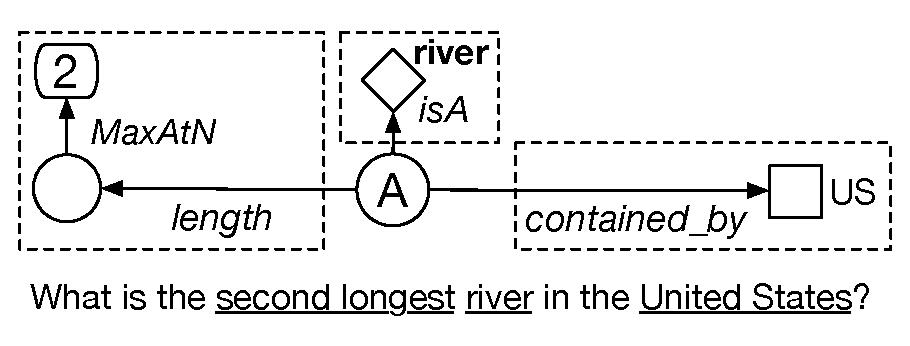
\includegraphics[width=0.4\columnwidth]{figure/schema/intro.eps}
\bicaption{二元关系 ``has grandfather'' 的语义表示。}{An example schema graph.}
\label{fig:schema-intro}
\end{figure}

具体而言,给定自然语言中的关系$r$以及抽取出的三元组$(e_{subj}, r, e_{obj})$,
本章的研究任务是在知识库中挖掘出一系列与之相关的模式图,
并且用概率分布的形式,描述用特定模式图代表该关系语义的可能性。
%The schema representation is formed in a tree structure, which
%consists of the predicate path connecting two entities directly,
%and constraint predicates at the branch of the path.
%Therefore, our paraphrasing task is the generalization of previous
%path-based work.
%This generalization is important because complex relations that
%require constraints constitute a non-trivial portion of
%all extracted relations from open IE.
%For example, by manual inspection, out of 2,500 most popular
%relation patterns in PATTY dataset,  13\% of the relation instances
%%and 7.5\% \KQ{18\% in our experiment} of relation patterns
%are actually complex (i.e., require more than a simple path to represent the semantics).
在进行模式图推理的过程中,我们主要会面临以下三个技术性挑战:

首先,候选模式图的数量非常庞大。
传统的规则推导中只考虑谓词路径,虽然候选路径的数量随长度呈指数增长,
但在知识库中能够连接两个特定实体的路径仅有少数,
因此简单遍历可以得到所有的候选路径。
然而,具有树形结构的模式图中,不仅存在额外的谓词作为分支,
而且包括用于语义限制的实体,任何一个实体的改变,都会产生一个新的模式图。
若使用暴力枚举生成模式图,时间复杂度上无法承受,
同时还会生成大量偏离语义的模式图。

其次,模式图推理需要做好粒度上的平衡。
当一个模式图缺少足够的语义限制,它虽然能匹配已知的三元组,但也可能混淆了错误的三元组。
反之,若一个模式图包含了不必要的语义限制,就很可能无法匹配已知的三元组。
很显然,太具体或宽泛的模式图都无法精确表示一个关系的语义,
但是如何兼顾这两点,并通过概率分布描述不同粒度候选的语义匹配程度,
这成为了模式图推理过程中的另一个难点。

最后,模式图推理模型仅有三元组作为训练数据,
不存在标注好的模式图,同时没有明确给出不符合特定关系的错误三元组数据,
这给学习过程增添了难度。
一种规避方法是使用封闭世界假设(Closed World Assumption),
即假定所有未见过的三元组都是错误的。
但考虑到知识库本身远不够完整,封闭世界假设会带来大量的错误反例,
这并不是一个最好的解决方案。

%In general, simpler schemas tend to be more general in meaning,
%whereas more complex schemas are more specific in meaning.
%A schema that is too general is less expressive and less informative,
%while a schema that is too specific may not be able to cover all
%the entity pairs.

%We define the notion \textbf{simple schema}, if the schema graph cotains \textit{only}
%a path of predicates connecting entities from $e_1$ to $e_2$ in the knowledge base.
%To this end, state-of-the-art systems have been proposed for solving this task.
%

%2. what's knowledge base try to do
%Structured knowledge base (KB) is a graph based taxonomy containing real world
%entities,  types,  binary predicates between entities and ``IsA'' relations
%between entities and types.
%(Machine readable, containing millions / billions of facts)

%Structured KBs such as WordNet \cite{miller1995wordnet},
%Yago \cite{suchanek2007WWW} and Freebase \cite{bollacker2008freebase} are widely used in information extraction
%and semantic learning tasks. In order to make relation schemas understood by human, we leverage types
%in the KB as the output of relation schemas.

%3. what to do is to extract schema
%The paraphrasing task is to map a natural language relation into structured
%canonical forms in KB, which is understood by both machine and human.
%
%We call the representation as \textit{relation schema} throughout this paper.
%
%\KQ{how to give a clear impression on schema}
%%\cite{bollacker2008freebase}
%%%Figure show schema on FB as the first impression (mention FB's size here)
%informal
%One can see that a relational schema is a template of many subgraphs
%with the concrete structure in the knowledge base.
%The goal of this paper is to enable effective and efficient translation
%process, which we call ``paraphrasing.''


%add. why we need to schema
%Paraphrasing is a open task, since the structured schema is an important knowledge
%used in many down-stream applications, such as question answering, text entailment
%and short text similarity querying.
%(Arguing)

%1. why we need paraphrasing

%2. what's the advantage of schema
% SPARQL query
% user intent query (check view synthesis paper)
%Paraphrasing is a fundamental task in natural language processing and understanding,
%especially in the system of question answering ,
%and knowledge base completion.
%In these tasks, the relation coming from input sentence (or question) is transformed
%into semantic structure in the knowledge base, and the overall accuracy is largely
%determined by the quality of the structural representation.
%
%
%There are three main advantages for our schema based model.
%First, each schema is an independent structure that represents the target relation.
%Feature weights produced by discriminative model can tell us which schemas are more
%suitable for the relation, while a single feature snippet is less expressive.
%Second, the schema is a subgraph of a semantic knowledge base.
%Our system can easily transform a schema into a SPARQL query due to the widely used RDF model
%in semantic knowledge bases. Therefore, an end-user can query RDF to retrive instances
%or a natural language relation, even though they don't know how to write a SPARQL query.
%Third, the schema is human-readable. Interactive online QA systems can display schemas and
%allow end-users to adjust them, leading to a better user experience.
%
%

%4. claim the gap between kb and nl on description
%Recap the semantic gap between relations and knowledge base predicates that we mentioned
%Yet some knowledge base is lack of predicates, however, the gap couldn't be removed,
%even for Freebase containing thousands of binary predicates.
%%5. simple exmple & chain example (mediator)
%%6. branching example
%%a) place_of_birth v.s. <people, was born in, place>
%%b) mediator: film.actor.film --> film.performance.film   v.s.   "starring in"
%%c) branching: female spouse v.s. "wife of"
%The predicate name ``place\_of\_birth'' in \figref{fig:fb-schema} (a) shows the difference,
%compared with relation words ``was born in'';
%\figref{fig:fb-schema} (b) brings the gap to structural level, where the schema shows a
%complex ``parent + parent + male'' style, even ``grandfather'' relation is so common in
%the real world; Meanwhile, \figref{fig:fb-schema} (c) show that the schema must include
%a intermediate node (used to maintain the ternary relation ``actor plays a character in a film'').
%These varieties make the paraphrase task challenging.
%
%%traditional method & limits
%%0. informally, composite relation
%%(Lei Zou) (EMNLP 2011) (AAAI 2012) (Tran 2009) (EMNLP 2015)
%For the part of feature based supervised systems, the first branch is graph-walk based
%\cite{lao2010relational,lao2011random}, a candidate schema is drawn from the predicate path
%between some entity pairs, and the probabilistic distribution of random walking from $e_1$
%to $e_2$ in KB on the schema is used as a feature to train the importance of each path.
%The second branch is logic based \cite{zhang2012ontological}, where the system uses hand
%crafted soft rules to mine various features that leads to good relation schemas.
%Since soft rules are fixed and independent of relations, the dimension of feature space
%is limited.
%
%Besides, unsupervised models are also used. Zou et al. \cite{zou2014natural}
%followed the idea of TF-IDF score \cite{blabla} to calculate the best schema with respect to a
%speicifc relation. While different input relations could have overlap meaning, this situation
%causes a lower score of schemas representing the overlapping part.
%
%In addition, among all different paraphrasing solvers, the process of candidate schema
%searching could always be a big challenge. All systems discussed above only generate
%simple schemas (predicate paths), which is also a limitation for searching more
%specific and meaningful schemas.
%
% our approach
%1. IMPORTANT data-driven

%TODO:我觉得这里要加一段,可以稍微提到approach里面的东西,总之就是为了应对xxx,我们xxx。
%不是bullet的形式。
%啥是LP,TC,啥是高效剪枝,啥是具体的生成模型,这些都可以写啊!!!!!!

本章提出的基于模式图的规则推导模型旨在解决应对以上三个挑战,
其主要贡献可以分为以下四个部分:
\begin{enumerate}
\item{我们定义了自然语言关系的模式图。
和传统规则推导模型相比,模式图是谓词路径形式的规则扩展,
通过挖掘隐藏的关联实体,在路径之上构建分支,
准确描述关系的复杂语义;}
%(\secref{sec:schema-problem});}
\item{我们提出了一种基于局部搜索的启发式方法,通过高效的剪枝策略,
快速生成关系所对应的候选模式图;}
%(\secref{sec:schema-candgen});}
\item{我们提出了一种基于数据驱动的方法,将模式推理问题转化为
查询任务进行建模,并在不明确生成负面训练数据的情况下,
学习候选模式图之间的概率分布,实现不同粒度模式图的统一比较;}
%(\secref{sec:schema-inference});}
\item{我们对自然语言关系以及知识库中已有的谓词进行了知识库补全任务的测评,
包括主宾语预测和三元组分类两个子任务,
我们的模型在这两个测评任务上均显著优于已有方法。
具体生成的模式图结果表明,我们提出的模型能够挖掘出具体且精确的语义。}
%(\secref{sec:schema-exp})。}
\end{enumerate}


%  This paper addresses these challenges and makes the following contributions.
%  %We present a distant-supervised learning approach to solve the
%  %paraphrasing problem, with the following contributions:
%  \begin{itemize}
%  \itemsep0em
%  \item We define schemas as a generalized representation of natural language
%  relations in knowledge base (\secref{sec:problem});
%  \item %Due to the prohibitive space of possible schemas,
%  We present an effective local search based heuristic to generate a set of
%  candidate schemas (\secref{sec:candgen});
%  \item We propose a data-driven approach to model the schema inference
%  problem as a querying task, and thus compute the probability distribution over schemas,
%  given a natural language relation and its instances
%  without explicitly generating negative training data (\secref{sec:schema});
%  \item The framework significantly outperforms
%  previous best approaches on link prediction and triple classification task.
%  The example results show that our schema inference model
%  is able to discover concrete and precise semantics (\secref{sec:eval}).
%  %and question answering. Furthermore, our schema representation is
%  %on par with the popular word embedding model in computing relation similarity (\secref{sec:eval}).
%  \end{itemize}


%# -*- coding: utf-8-unix -*-
% !TEX program = xelatex
% !TEX root = ../thesis.tex
% !TEX encoding = UTF-8 Unicode

\subsection{相关工作}
\label{sec:schema-related}

%\KZ{First discuss AAAI 2012 and EMNLP 2015, their pros and cons and how
%we stack up with them. Then discuss other less similar work. Finally
%applications that can benefit from this work, eg. QA, etc.}
% introduce AAAI2012, analyze pros and cons
%is based on such a procedure called ontology mapping. Given a user-specified relation along with its labeled instances, ontology mapping actually generates several complex SQL expressions over types and relations on the KB's schema. This procedure is quite difficult since the space of possible SQL views can be extremely large. In order to reduce the search space and select the best views, the authors first generates several constraints (hard rules) described in Markov Logic. This step actually is the a procedure to generate simple candidates schemas. Then, the probability of mappings is described using Markov logic Network after adding different rules into the network. Through weight training and relaxing the optimization problem to a linear problem, those candidate schemas with a high probability form to the mapping result. This work is able to show a set of best schemas for a target relation. However, the authors add several hand-crafted soft rules to Markov Logic Network which limits the dimension of feature space. Besides, the complex SQL views can actually be transformed to simple schemas (paths) which can not be able to handle complex relations in natural language form.
% introduce emnlp 2015 SFE


%Previous work~\cite{zhang2012ontological,gardner2015efficient,gardner2014incorporating,lao2011random} has attempted to map a relation to
%background KB skeletons.
%The goal of these works is to complete the imperfectly extracted KB
%\textit{NELL} \cite{carlson2010toward} by predicting all concept $b$
%which potentially have the relation $R(a, b)$ given a concept $a$.


%However, all of the above work only
%considers the simple path representations.
%In contrast, our approach adopts complex schema
%with constraints, which can describe more sophisticated NL relations.
%Moreover, when solving KB completion problem, we use only schemas
%of NL relations as features, whereas previous work use many other
%features.

随着大规模结构化知识库的提出与广泛使用,知识库补全任务成为了近年来的热门研究课题。
该任务旨在对知识库中已有的谓词进行建模,
通过预测潜在的($e_1$, $p$, $e_2$)三元组,实现扩充知识库的最终目的。
%Lao et al. \cite{lao2011random} proposed Path Ranking Algorithm (PRA),
%which used a random walk path finding algorithm to infer new relation instances by
%mapping the target KB relation into a path of several basic relations.
%The state-of-art system \cite{gardner2015efficient}
%examined the disadvantage of PRA and proposed a technique called subgraph feature extraction (SFE).
%It first runs local search to characterize the subgraph around each input entity in KB.
%Then SFE runs a set of feature extractors over these subgraphs to retrieve
%structural and semantic features for each candidate node.
%SFE outperforms other KB completion methods as it used more advanced features.
% embedding approaches
到目前位置,在该课题上的研究方法主要分为两类:
基于知识库表示学习和基于规则推导。
%By far most literature fall into two categories: {\em embedding} based and {\em rule} based.

知识库表示学习受到词向量技术\cite{mikolov2013exploiting,pennington2014glove}的启发,
将知识库中的实体类比为单词,
每个实体具有一个向量表示,对应连续语义空间上的一个点。
作为连接不同实体的桥梁,知识库中的每个谓词都对应着各自的向量或矩阵表示。
通过定义不同的向量或矩阵之间的运算方式,这类方法可以计算每个三元组的置信度,
以此实现对实体及谓词的表示学习。

RESCAL模型\cite{nickel2012factorizing}是一个基础的知识库向量模型,
它基于实体向量和谓词矩阵表示的双线性运算。
HOLE模型\cite{nickel2015holographic}是RESCAL模型的改进,
使用向量循环平移的技巧计算实体间的组合语义向量,大幅度降低了谓词的表示维度。
在众多知识库表示学习的方法中,有一组方法称为隐距离模型,
它们对三元组置信度的计算方式主要基于连续空间中的距离度量:
将主宾语向量经过某种方式的映射(翻译)之后,距离越小,置信度越高。
最典型的研究工作为TransE,其核心思路在于尽可能使每个三元组(h,r,t)
对应的向量计算满足$\textbf{h} + \textbf{r} \simeq \textbf{t}$,
即利用谓词向量将连续空间中的主语进行平移,使其尽量与宾语重合。
为了能更好地表示多对多的关系,相关文献\parencite{wang2014knowledge,lin2015learning}   %TransH, TransR
对TransE模型进行了改良。
%TransG,pTransE,sTransE,甚至更多自己还没听过的
%TODO:如果需要填充,这个可以在外面的Related Work里面多说一些。
% KALE, TEKE, HOLE
Wang等人提出了TEKE模型\cite{wang2016text},它对已有的翻译模型进行改良,
充分利用结构化文本的知识,寻找三元组中单词级别的共现,
并利用共现上下文微调实体和谓词的向量表示。


% too detailed
%In TransE, $\textbf{h} + \textbf{r} \simeq \textbf{t}$ is expected whenever triplet $(h, r, t)$ exists, and a loss function of $\sum_{(h,r,t)} \sum_{(h^{'},r,t^{'})} [\gamma + d(\textbf{h} + \textbf{r}, \textbf{t}) - d(\textbf{h'} + \textbf{r}, \textbf{t'})]$ is minimized during training, where $\gamma$ is the margin hyperparameter, $d(\cdot)$ is certain dissimilarity measure, $(h, r, t)$ is the true triplet and $(h^{'}, r, t^{'})$ are the corrupted triplets. TransH addressed TranE's problem in modeling 1-to-N, N-to-1 and N-to-N relations. It allows an entity to have different distributed representation when involved in different relations. TransH models each relation as a vector on a hyperplane, and when calculating dissimilarity, $\textbf{h}$ and $\textbf{t}$ are first projected onto that relation's hyperplane, then compute $d(\textbf{h}_{\bot} + \textbf{r} - \textbf{t}_{\bot})$. TransR~\cite{lin2015learning} proposed to represent entities and relations in distinct spaces, with translation performed in the relation space. For each relation $r$, TransR sets a projection matrix $\textbf{M}_r$ to project entity vector into relation space, i.e. $\textbf{h}_r = \textbf{hM}_r$, $\textbf{t}_r = \textbf{tM}_r$, and dissimilarity is computed as $||\textbf{h}_r + \textbf{r} - \textbf{t}_r||^2_2$.
%Other embedding methods include SME~\cite{bordes2012joint}, RESCAL~\cite{nickel2012factorizing}.

%TODO:这段不够严谨,需要靠外部Related进行补充,怎么着得讲清楚
基于规则推导的方法旨在用逻辑规则的形式表达谓词的语义。
例如$\text{parent}(x, y) \land \text{parent}(y, z) \rightarrow \text{grandparent}(x, z)$
是一个常识性的规则,我们可以通过规则的左侧部分,在知识库中寻找出更多的祖孙间的关系。
Jiang等人的工作\parencite{jiang2012learning}基于马尔科夫逻辑,通过挖掘的规则
对自动构建的知识库进行信息过滤。
其它一些方法使用概率软逻辑或关联规则挖掘完成类似的任务\cite{pujara2013large,volker2011statistical}。
%Pujara et al.~\cite{pujara2013large} proposed to use probabilistic soft logic (PSL) for this job.
%V\"olker et al.~\cite{volker2011statistical} proposed a statistical approach to induct schemas based on association rule mining.
Gal\'arraga等人提出的AMIE\cite{galarraga2013amie}以及AMIE+\cite{galarraga2015fast}系统
则直接根据知识库的三元组寻找置信度较高的一阶逻辑规则。
%TODO:妈呀我在说什么?
%TODO:上面这些研究感觉不属于KB的范畴,需要对它们进行一个概括,就这么放在这里肯定是不好的
%TODO:拟放进外面Related的东西:一个古老的论文(不一定是AMIE),PRA/SFE
最新的一些研究着眼于在知识库中寻找路径形式的规则,%为什么,得给一个理由吧
通过挖掘大量可能的路径,作为表示语义的特征。
Lao等人提出了PRA模型\cite{lao2011random},
通过在谓词路径上的随机游走策略,衡量其连接一对实体的好坏程度,
目标关系的语义等同于不同路径特征的带权组合。
Gardner等人对PRA模型进行改进,提出了SFE模型\cite{gardner2015efficient},
除了捕捉连接主宾语的路径以外,还从主宾语各自的知识库子图中挖掘独立的特征,
同时谓词路径的定义更加宽泛,允许在其中使用通配符表示任意谓词。
此外,Wang等人提出了CPRA模型\cite{wang2016knowledge},
这是对PRA模型的另一种改进,
通过挖掘目标关系中的相关性,使得相似关系之间的路径挖掘结果可以互相影响。
然而,通过开放式信息抽取获得的三元组数量相对有限,
不同的关系之间几乎不存在重叠的实体对,在这种场景下,
CPRA模型效果等价于原始的PRA模型。

%  Other works treat rules as paths through entities in the KB.
%  %Path based methods infer connections between entities from existing paths in the KB.
%  Lao et al.~\cite{lao2011random} proposed Path Ranking Algorithm (PRA),
%  which used a random walk path finding algorithm to map the target KB relation into a sequence of several basic relations.
%  Subgraph feature extraction \cite{gardner2015efficient}, known as SFE, explores more than paths in the KB 
%  by exploring structural features around entities, and allows using a wildcard to indicate any possible edges.
%  %. It first runs local search to characterize the subgraph around each input entity in KB, then SFE runs a set of feature extractors over these subgraphs to retrieve structural and semantic features for each candidate node.
%  Wang et al.~\cite{wang2016knowledge} improved PRA with Coupled Path Ranking Algorithm (CPRA),
%  where similar relations are clustered and jointly learned.
%  However, in the experiment setting of this paper, relations in OpenIE dataset usually do not overlap and CPRA degenerates to PRA.

一些相关的研究尝试在知识库向量学习的基础之上加入一定的逻辑规则。
Guo等人提出了KALE模型\cite{guo2016jointly},其主要思想是将规则转换为多个三元组之间的与或非逻辑操作,
因此基于翻译模型计算的三元组置信度得以在逻辑规则级别产生交互。
TRESCAL模型\cite{chang2014typed}在经典的RESCAL模型中加入了知识库的类型限制。
%TODO:Rockt\"aschel et al.~\cite{rocktaschel2015injecting} proposed to embed first-order logic into low-dimensional vector spaces,
而Wang等人的工作\cite{wang2015knowledge}使用整数线性规划技术,将知识库向量表示和规则挖掘进行统一,

%Some works in KBC combine above approaches by incorporating rules into embedding models.
%Logic rules are combined with embedding in KALE \cite{guo2016jointly},
%where the idea is to represent and model triples and rules in a unified framework.
%TRESCAL~\cite{chang2014typed} encodes type constraints into RESCAL~\cite{nickel2012factorizing}.
%Rockt\"aschel et al.~\cite{rocktaschel2015injecting} proposed to embed first-order logic into low-dimensional vector spaces,
%and Wang et al.~\cite{wang2015knowledge} integrated KB embedding and rules with integer linear programming (ILP),
%with the objective function derived from the embedding model and constraints translated from rules.

狭义的知识库补全任务只考虑知识库中的谓词,
我们的工作将知识库补全的场景进行了扩展。
考虑到为了降低知识库结构与自然语言描述的差距,
知识库补全任务也可以针对自然语言中的二元关系。
开放式信息抽取与这样的任务相契合,
既提供了全新谓词,又有一定量的三元组用于补全学习。
一些已有的工作也关注了自然语言关系到知识库的映射。
Zou等人的工作\cite{zou2014natural}使用了非监督学习的方式,
利用TF-IDF特征寻找关系到谓词路径的匹配。
Zhang等人的工作\cite{zhang2012ontological}
利用马尔科夫逻辑网络\cite{richardson2006markov},
学习自然语言关系对应于不同候选谓词路径的概率。
这些方法对关系的表示局限于路径的形式,
无法准确地描述一个形式简单但具有组合语义的关系。
我们的工作旨在理解具有复杂语义的关系,挖掘其包含的隐含限制条件,
并通过具有 ``{路径+分支}'' 结构的模式图进行语义建模。


%  In traditional KBC tasks, the target relation is an existing predicate in the KB,
%  while we extend the definition of KBC into a broader scenario, since one may wish to add
%  a new predicate (derived from natural language) into existing KB, and the Open IE system
%  can help provide seed relation instance for further enrichment.
%  In terms of mapping NL relation into KB, Zou et al.~\cite{zou2014natural} proposed an unsupervised TfIdf-based algorithm to figure out the mapping confidence of predicate paths to one relation.
%  %The algorithm adopted the idea of tf-idf, which combines entity pairs covered by the path
%  %in a relation (as term frequency)
%  %and the number of distinct relations that one path could support (as inverted document frequency).
%  Zhang et al.~\cite{zhang2012ontological} also focused on learning path predicates using a Markov Logic Network~\cite{richardson2006markov}.
%  %which consists of soft rules
%  %on both positive and negative entity pair coverage, along with length of paths.
%  While the above KBC systems focus on path representation, our work aims at understanding
%  semantically complex relations and adopts complex schema with constraints.






%Natural language relations always have more complex meaning
%than KB predicates and using our system,
%a target human raised relation can be mapped into an
%explicit readable schema graph.

%To solve the paraphrasing problem between natural language relations and KB predicates, we aim to represent a human raised relation with several explicit schemas. One major difference between our technique and others is that during the procedure of generating candidate schemas for target relations, we do not limit the schemas to be simple only. We fully utilize the information of KB, adding extra constraints to the simple schemas and resulting in more complex schemas. Specifically, we perform a breadth-first search to construct the skeleton of a specific relation schema which is similar as the path finding procedure in the previous works \cite{gardner2015efficient,gardner2014incorporating,lao2011random,zhang2012ontological}. Beyond relation path, we use a depth-first search to further add more information attributes to the relation path generated in the first step and transform it into a more specific and complex graph form, under the guidance of \textit{Minimum Description Length} (MDL) \cite{fisher2008dirt,grunwald2007minimum} principle. MDL principle is used as a trade-off since it measures the cost of transmitting both schemas and entity pairs.

% query synthesis

% question and answering via paraphrasing
%% remove QA
%Our work also intersects with ontology question answering.%~\cite{yahya2012natural,krishnamurthy2012weakly,fader2013paraphrase}.
%One branch of QA techniques are semantic parsing based, it translates questions directly into structural query graphs through pre-defined grammars, such as CCG~
%\cite{kwiatkowski2010inducing,cai2013large,kwiatkowski2013scaling,reddy2014large}
%and $\lambda$-DCS~\cite{liang2011learning,berant2013semantic,berant2014semantic}
%, then perform query on SPARQL engine.
%Our schema shares the similar backbone structure with query graph, but the key difference between
%semantic parsing and our work is how to generate the query graph:
%In semantic parsing methods, the query graph is constructed recursively based on combining syntactic components,
%therefore complex semantic can only be generated if the question is \textbf{syntactically} complex;
%therefore complex semantics is limited to \textit{syntactically} complex questions;
%in contrast, we leverage grouped training data to discover semantic representation
%for syntactically simple but \textit{semantically} complex phrases.

%Another branch of QA techniques are information retrieval based~
%\cite{yao2014information,bordes2014question,yih2015semantic},
%which first retrieves a broad set of candidate answers or query graphs by traversing around
%question focus entity over the knowledge base, and then design syntactic and semantic features
%to capture the latent associations between question surface and the answer.
%Closest to our schema generation method is Yih et al.~\cite{yih2015semantic} who also
%uses depth-first search method to extract candidate query graphs.
%However, their constraints relied on handcrafted rules with explicit syntactic components,
%and are available only in certain domains (such as gender, marriage and event time).
%While our method is able to summarize more flexible constraints from existing relation instances.

%Besides, our work is similar to query synthesis in relational database~\cite{niehren2013query,das2010synthesizing,cheung2012inferring,cheung2013optimizing}.Given a set of input table and an output table,query synthesis automatically produces a relational query that produces the output when applied to the input.This problem is similar to ours as the query is analogous to the schema while the database is similar to the KB, but the database query is more close to a decision tree, because the task requires producing the exact output table. Typically, Zhang and Sun \cite{zhang2013automatically} address query synthesis using a three-steps technique. First they create an incomplete query skeleton which captures the basic structure of the result query, then complete the skeleton by adding some concrete and accurate rules and generate a list of candidates, and finally ranks the candidates, which simply prefers queries with simpler structures. Though first two steps share the same intuition with our schema generation procedure, the techniques cannot be directly applied to NL domain, due to the different functionalities between relational query and schema.

%In question answering by paraphrasing \cite{harabagiu2006methods,berant2013semantic,fader2013paraphrase,kwiatkowski2013scaling,berant2014semantic},
%as a representative, Berant and Liang~\cite{berant2014semantic} attack
%semantic parsing by mapping natural language utterances into logical forms
%to be executed on a KB using a paraphrase model and furthermore
%improved QA performance. We compared our results to theirs in the experiments
%section.

% other parts
%Other related work includes unsupervised systems such as
%\cite{zou2014natural}, which calculates scores of candidate skeletons
%using TF-IDF and then choose the best one to represent the target relation.
%%As for concrete mapping format, MapOnto \cite{an2006discovering} uses Horn clauses when produces mapping rules between two schemas. Others \cite{zhang2012ontological} generate complex SQL queries consisting of operations like join, union, project and select as mappings.
%Graph-based representations \cite{reddy2014large} is usually
%used in exploiting structural and conceptual similarity between NL
%and KB. Zou et al. \cite{zou2014natural} interpret a natural language
%question as a semantic query graph where each vertex represents an argument
%and each edge is associated with a relation phrase.
%Compared to these works, our schema graph is more complex with constraints.


%# -*- coding: utf-8-unix -*-
% !TEX program = xelatex
% !TEX root = ../thesis.tex
% !TEX encoding = UTF-8 Unicode

\subsection{任务定义}
\label{sec:schema-problem}

%In this section, we first give formal definitions of the knowledge base
%and the schema graph, then describe the paraphrasing task.

%TODO: definition的样式没了,不过不一定需要。
\begin{definition}

在本章中,我们定义知识库为$KB=\{E, L, P\}$三部分组成,具体如下:
$E$为知识库$KB$中所有实体集合;
$L$为$KB$中所有不同谓词的集合;
%  All the entities, types and predicate names in $KB$ are identified by a unique id.
$P$为$KB$中所有事实三元组集合,
每一个三元组表示为$p(e_1, e_2)$,其中$e_1, e_2 \in E$,并且$p \in L$.
此外,知识库中存在用于描述一个实体所拥有类型的谓词$IsA$,
为了简化描述,本章中我们将不同类型也看做实体,同属于集合$E$中。

\end{definition}

%\KQ{Add some sentences showing what's a schema: abstraction}

%1. relation comes from a detail subgraph (give an example of mo_of)
%A knowledge base is capable of representing complex relations
%between real entities.
%As what we've shown in \figref{fig:fb-schema}, though there is no
%direct grandfather relation between ``Pactrick Schwarzenegger''
%and ``Gustav Schwarzenegger'', they can be indirectly connected via
%the ``parent + parent + male'' structure.
%2. relation schema is a summarization o a list of subgraphs. (by substitution)
%Intuitively, different instances of a complex relation type share a
%common structure (the schema), which is the template of that relation.
%Now we give the formal definition of a schema graph.


%3. formal def. of S
\begin{definition}


一个模式图$S$同样由三部分构成,$S=\{E_S, X, P_S\}$,具体如下:
$E_S \subseteq E$,为模式图中出现的具体的实体集合;
$X$为实体变量的集合,每一个变量$x \in X$在模式图中等同于占位符,
为特定实体$e \in E$的抽象;
模式图中包含两个特殊变量,即$x_{subj}, x_{obj} \in X$,
分别代表目标关系的主语和宾语实体;
$P_S$为模式图中的抽象三元组集合,每一个抽象三元组为$p_s(v_1, v_2)$,
其中$v_1 \in X$ , $v_2 \in E_S \cup X$ 以及 $p_s \in L$。
此外,模式图$S$具有以下性质:
\begin{itemize}
  \item $S$的表现形式为有向树形结构,且根节点一定为主语的实体变量$x_{subj}$;
  \item 连接主语变量$x_{subj}$和宾语变量$x_{obj}$的谓词路径,称为模式图$S$的骨架;
  \item 骨架之外的所有抽象三元组称为模式图的限制(或分支);
  \item 一个仅具有骨架而不包含任何限制的模式图,称为简单模式图,等价于谓词路径。
%   \KZ{How do you ensure that
%	all nodes internal nodes are variables and all external nodes are
%	are constants or $x_1$ or $x_2$. Also how do we say that there's no
%	two consecutive variable nodes in the tree. These are not clear now.}
%  \item On the path from $x_1$ to $x_2$ (which is the skeleton
%        of $S$), all vertices $v \in X$.
%  \item In the tree, all non-leaf vertices $v \in X$.
%  \item[-] $c = \text{solid}$, if and only if $v_1, v_2 \in X$, $p_s \in L$,
%  \item[-] $c = \text{dashed}$, if and only if $v_1 \in X, v_2 \in E'$, $p_s \in L$,
%  \item[-] $c = \text{isa}$, if and only if $v_1 \in X, v_2 \in T'$ and $p_s = \text{isa}$.
\end{itemize}
%\KZ{I think the input $e_1$ and $e_2$ should be separated from E'. These
%are the target entities, different from other concrete entities in the
%schema.}
  %These restrictions make every predicate in $S$ connecting to at least one variable.
  %Generalize the definition. We do not need the graph to be a tree.

  %\item[*] All $solid$ predicates form a tree, where both $x_{subj}$ and $x_{obj}$ must
  %be a leaf, that is, linked by only one $solid$ predicate.
\end{definition}

\begin{figure}[ht]
    \centering
    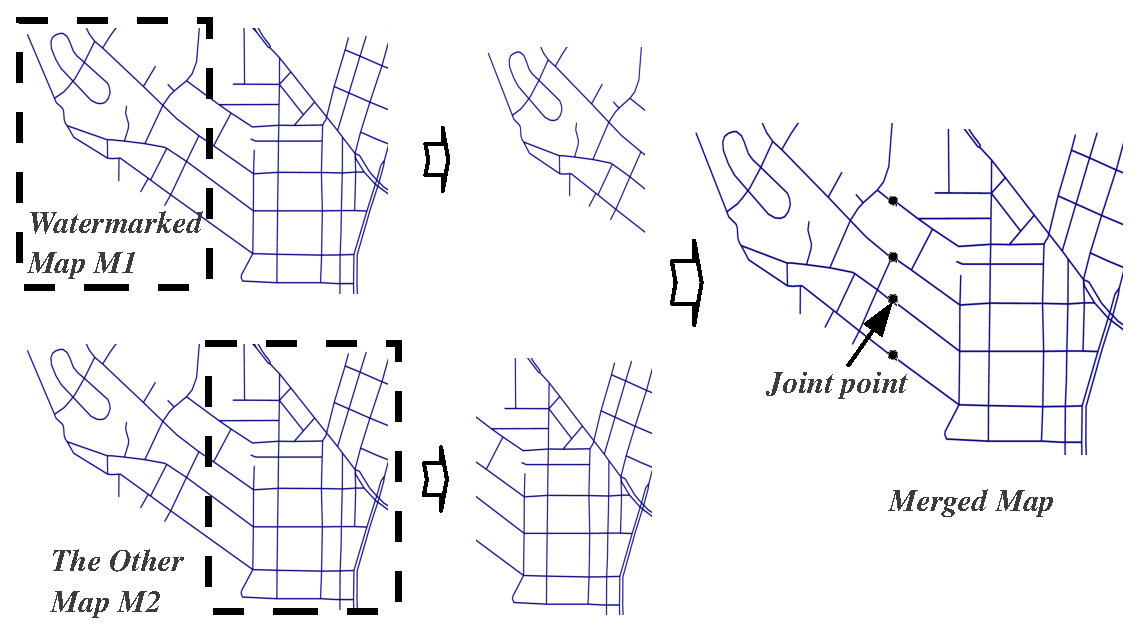
\includegraphics[width=0.5\columnwidth]{figure/schema/problem.eps}
    \bicaption{模式图的一般形式。}{A general style of a schema graph.}
    \label{fig:schema-problem}
\end{figure}


\figref{fig:schema-problem}显示了模式图的一般形式。
%可以讲一下E_S, X, P_S分别是啥。
可以发现,其中的每一条边都至少连接了一个实体变量。
模式图代表着知识库中,满足相同特定结构的一系列具体子图。
这些具体子图称为实例图(Grounded Garph),作为模式图的实例化形式,
所有的实体变量$x_i$被替换为特定的实体$e_i \in E$,
且每一个抽象三元组$p_s(v_1, v_2)$在实例化之后均对应
存在于知识库中的事实$p(e_1, e_2) \in P$。
例如\figref{fig:schema-intro}中的模式图,
其不同的实例图囊括了知识库中所有已知的(个人,双亲,双亲父亲)知识。
对于实例图中的主宾语对$(e_{subj}, e_{obj})$,
我们称其为模式图的一个支持实例。
%我们称该实体对支持当前的模式图。%TODO: 换个说法?
%If a ground graph of $S$ instantiates $x_{subj}$ to $e_{subj}$ and $x_{obj}$ to
%$e_{obj}$, then $S$ is said to {\em cover} the entity pair 



根据以上符号定义,
给定知识库$KB$,自然语言关系$r$以及多个关系三元组\{($e_{subj}$, $r$, $e_{obj}$)\},
我们对关系的深度语义挖掘任务为,
推导出一系列描述其语义的候选模式图,并学习模式图上的概率分布,
以此表示自然语言关系所具有的多义性。
%induce a list of schemas and the probability distribution over the schemas, such that observed instances
%can be produced with the highest probability.

%find a ranked list of schemas that have the most similar meaning
%to $r$. \KZ{Why isn't the problem one that finds a list of schemas
%that {\em collectively cover} as many input pairs as possible?}

%The weight of each schema represents the fitness score over inputs.
%Intuitively, schema fits input entity pairs properly, if neither too general
%(producing too many coverages),
%nor too specific (only covers a few positive pairs).

%It's clear that output schemas could be selected from any schema covered at least one entity pair.
%However, existing knowledge base could have millions of entities and thousands of different
%kinds of predicates, leading to a huge search space.
%The searching direction is crucial for finding more suitable schemas within
%limit time and space.
%In addition, with no labeled schemas as training data, we need a
%data-driven metric to label each schema with a ``silver'' score, measuring
%the quality of one candidate schema.
%Therefore, we define a function $cost(EP, S)$, measuring the cost of one schema $S$
%with respect to positive input pairs $EP$, and then perform a local search algorithm guided by this function.
%\KZ{Shall we give a more formal def of the paraphrasing problem? You can
%refer to the way it's defined in Gong yu's paper. It's similar.}

%Next, we present an overview of the framework (\secref{sec:approach}),
%and explain how candidate schemas are generated (\secref{sec:candgen}),
%and how the schema probability is computed based on relation instances (\secref{sec:schema}).
%

%and how the silver score is computed to train the classifier for
%schema inference.

%how we obtain the cost function based on the view of information theory (\secref{sec:scoring}),
%and how the local searching process is performed (\secref{sec:candidate}).

%In section 3, we focus on how we build th   based on the view of information theory.
%
%For the local searching algorithm,
%
%Output schemas are chosen from a set of \textit{candidate schemas} in KB,
%which are the most suitable (neither too general nor too specific) for the given data.
%
%In order to describe all given entity pairs, the hit pairs of output schemas
%must cover all the given entities.
%Furthermore, we build a cost function to measure the fitness score over a schema and entity pairs,
%turning our task to an optimization problem.
%%2. bridge the gap bet. entity and schema. that's assign
%%A ground graph bridges the gap between $\langle e_{subj}, e_{obj} \rangle$ and a schema.
%%All schemas that can hit at least one entity pair form the schema searching space.
%%Each entity pair is assigned to at least one schema which hits the pair.
%%After the step of assignment, a cost is produced when a schema is selected
%%to describe all its assigned entity pairs assigned.
%%%3. Goal: Min Cost
%%With cost function provided, we look for a set of schemas describing
%%all entity pairs at a minimum cost.
%
%%4. Formally Define.
%The following is the formal definition of our task.
%
%\begin{definition}[The Paraphrasing Problem]
%\label{def:pp}
%Given $KB$, entity pairs $EP = \{ep_1, ..., ep_n\}$,
%a cost function $f: EP \times S \rightarrow [0, +\infty)$,
%and a function $sel$ that selects all candidate schemas ($CS$) from $KB$,
%return a set of output schemas $OS \subseteq CS$, such that:
%\begin{itemize}
%    \item[-] $EP \subseteq \bigcup_{S \in OS} HP(S)$,
%    \item[-] Whole cost $Z = \sum\nolimits_{S \in OS} f(EP, S)$ is minimum.
%\end{itemize}
%%
%%Given $KB$, a binary relation pattern $rel$ with its support entity pairs
%%$EP = \{ ep_1, ..., ep_n \}$, cost function $f$ and $g$,
%%Let $CS = \{S | EP \cap HP(S) \neq \emptyset \}$ be \textit{candidate schemas} and
%%$DS = \{S_1, ..., S_m\} \subseteq CS$ be a set of \textit{selected schemas}.
%%Let $Ass_{m \times n}$ be an 0/1 \textit{assignment matrix} from $EP$ to $DS$ and
%%\textit{support set} $sup(S_j) = \{ep_i | Ass_{ij} = 1\}$ be all entity pairs assigned to the $j$-th schema.
%%The assignment $Ass$ is a valid assignment over $EP$ and $SG$ if it satisfies the following
%%constraints:
%%\begin{itemize}
%%    \item[-] $Ass_{ij} = 1 \Rightarrow ep_i \in HP(S_j)$,
%%    \item[-] $\forall ep_i \in EP, \exists S_j \in DS, Ass_{ij} = 1$,
%%    \item[-] $\forall S_j \in DS, \exists ep_i \in EP, Ass_{ij} = 1$,
%%\end{itemize}
%\end{definition}
%
%%The selected schemas $DS$ and corresponding $Ass$ are optimal, if it minimizes
%%the cost $Z(DS, Ass) = \sum\nolimits_{S \in DS} f(S) + g(S, sup(S))$ , where $f$ is a
%%cost function over a specific schema, and $g$ is a cost function over a schema along
%%with its support set. Both $f$ and $g$ are non-negative functions and defined by users.
%
%%Now we define the task of paraphrasing between NL and KB. Given KB, a binary relation
%%pattern $rel$ with its support entity pairs
%%$EP = \{\langle e_1^{(1)}, e_2^{(1)} \rangle , ..., \langle e_1^{(n)}, e_2^{(n)} \rangle \}$
%%from KB, we want to find a set of relation schemas $\vec{S}$ that:
%%
%%\begin{itemize}
%%    \item[-] Each entity pair is hit by at least one schema in $\vec{S}$,
%%    \item[-] The schemas fits $EP$ at the best (neither too general nor too specific).
%%\end{itemize}
%%
%%where the score of fitness is produced by a cost function $Cost(EP, \vec{S})$.
%%The cost function captures both compactness and precision for the set of schemas to describe the entity pairs.
%
%
%%\KQ{The reason of restricting at most K relation schemas is to avoid generating too many schemas.
%%In the formula, Cost(EP|S) is the dominant one,
%%probably 5~10 pairs hit by one specific schema could bring that schema into description set.}
%%
%%Next, we prove that the paraphrasing problem is NP-Hard.
%%We show that by constraining $sel$ and $f$ to some specific classes of
%%functions, the resulting instance of the paraphrasing problem can
%%be reduced from the well-known {\em weighted set cover problem},
%%which is NP-complete.
%%
%%\begin{theorem}
%%Given $KB$, $EP$, candidate selecting function $sel$ and cost function $f$,
%%computing the optimal output schemas for describing all pairs in $EP$, is NP-Hard.
%%\end{theorem}
%%
%%\begin{proof}
%%%Rephrase that a simplified instance of our problem is still NP-Hard.
%%We first state the simplified instance of the paraphrasing problem.
%%The function $sel$ is restricted by only returning a special kind
%%of schema, which has only $x_{subj}$ and $x_{obj}$ connected by a solid
%%predicate. In addition, the cost function $f$ is simplified as
%%$g: S \rightarrow [0, \infty)$, that is,
%%the cost is only determined by the schema, and not by EP.
%%
%%After the simplification, the \textbf{decision version} of the
%%paraphrasing problem is as follows:
%%Given $KB$, $EP$, $sel$, $g$ and a threshold $\theta$, is there a set of output schema $OS$
%%covering all pairs in $EP$, such that whole cost $Z \leq \theta$ ?
%%The proof relies on a reduction from \textsc{Weighted Set Cover} problem:
%%Given a universe $U = \{u_1, ..., u_n\}$, a threshold $\theta$, a set $V = \{v_1, ..., v_m\}$
%%whose union equals to $U$, each $v_j \subseteq U$ and a weight set $W = \{w_1, ..., w_m\}$ assigned to each $v_j$,
%%is there a cover $C \subseteq V$ whose union equals to $U$, and the summation weight is no larger than $\theta$ ?
%%
%%\textit{Reduction:} For an arbitrary instance of \textsc{Weighted Set Cover} problem,
%%we build a $KB$ based on $U$ and $V$, where it contains only $m$ different predicates $p_1, ..., p_m$,
%%leading to a set $m$ simple candidate schemas.
%%We map each $u_i$ to an entity pair $ep_i = \langle e_{subj}^{(i)}, e_{obj}^{(i)} \rangle $.
%%For any $u_i$ and $v_j$, if $u_i \in v_j$, we add a predicate instance $p_i(e_{subj}^{(i)}, e_{obj}^{(i)})$ into $KB$.
%%Finally, we define the cost function as $g(S_j) = w_j$ for each schema.
%%
%%Since all schemas have only one edge, retrieving candidate schemas from $KB$
%%along with hit pairs can be done in polynomial time. Therefore, the paraphrasing decision problem
%%is formulated as: Given $n$ entity pairs and $m$ sets of hit pairs whose union cover all pairs,
%%with the weight $w_j$ assigned to the $j$-th set, can I pick some sets that still cover all
%%the entity pairs, satisfying the summation weight no larger than $\theta$ ?
%%Obviously, solving this paraphrasing decision problem is equivalent to
%%solving the corresponding \textsc{Weighted Set Cover} problem.
%%\end{proof}
%%
%%%In this reduction, $U$ and $V$ are used to construct a $KB$,
%%%where $m$ different predicates $p_1, ..., p_m$ are in $KB$,
%%%each $u_i$ indicates an entity pair $\langle e_1^{(i)}, e_2^{(i)} \rangle $,
%%%and the relation instance $p_i(e_1^{(i)}, e_2^{(i)})$ is contained (or not) in $KB$
%%%according to whether $u_i$ is covered by $S_j$.
%%%Since we only consider the schema with one solid edge,
%%%the complexity of finding all \textit{candidate schemas} of these $n$ entity pairs
%%%is within polynomial time, where the $j$-th candidate schema hits those corresponding entity pairs within $V_j$,
%%%with the cost function $f(S_j) = w_j$.
%%%In addition, since the function $g$ is always zero, the assignment step could be ignored (if $S_j$ is selected,
%%%then all its hitting pairs would be assigned it without bringing extra costs).
%%%Therefore, if there exists a cover $C$ satisfying the $\theta$ limit, then
%%%it's possible to select schemas covering all entity pairs with cost no more than $\theta$.



%============================================================

\section{我们的方法}
\label{sec:schema-approach}

本节主要介绍将自然语言关系映射为模式图的具体方式。
给定关系$r$以及其一系列三元组作为训练数据,
我们首先依据给定的主宾语对($e_{subj}$, $e_{obj}$),
从它们支持的所有模式图中寻找可能性较高的候选模式图,
然后对具有不同粒度的模式图进行重要性衡量。
由于没有直接的\textless 关系,模式图 \textgreater 对作为训练数据,
我们提出了一种基于远距离监督学习的方式,
学习所有候选图上的概率分布。

%TODO: candgen可以多讲一些,为了凑IJCAI篇幅,这里的内容实在是有点少。
%# -*- coding: utf-8-unix -*-
% !TEX program = xelatex
% !TEX root = ../thesis.tex
% !TEX encoding = UTF-8 Unicode

\subsubsection{候选模式图生成}
\label{sec:schema-candgen}

根据已有的关系实例,我们提出了一种高效的搜索算法,
在知识库上挖掘可能表示关系语义的候选模式图。
其基本思路在于,首先通过主宾语对寻找仅由骨架(谓词路径)构成的简单模式图,
带有限制的模式图生成则以简单模式图为起点,
不断寻找与关系三元组契合的限制,
并通过递归的形式将新的限制连接到已有的候选上,
一步步生成具有复杂结构的模式图。

简单模式图的生成基于实体对在知识库中的直接连接。
我们使用双向广度优先搜索,为每个实体对提取由主语连接到宾语的所有谓词路径。
考虑到一个自然语言关系通常由短语构成,通常不会具有太多的语义跳跃,
因此我们对谓词路径长度进行限制,避免生成大量无意义的路径。
基于前人的工作\parencite{zhang2012ontological},
我们限制谓词路径最长不超过3。
%6. why use minimal coverage
此外,为了尽可能保证每一个候选图的质量,
我们需要排除那些仅由偶然数据生成,实则偏离语义的候选图。
一个有效的识别方式利用了候选图的支持率,
即支持候选图的实体对占目标关系所有已知实体对的比例,记做$sup(S)$。
我们在生成过程中指定支持率阈值$\gamma$,
并移除那些支持率$sup(S)$小于$\gamma$的模式图。
综上,对谓词路径和支持率的限制,可以使候选生成步骤过滤大量的干扰模式图。

\begin{figure*}[tp]
    \centering
    \includegraphics[width=1.0\columnwidth]{figure/schema/schema_gen-crop.eps}
    \bicaption{``has father'' 模式图挖掘示例。}{Candidate generation example of relation ``has father''.}
    \label{fig:schema-candgen}
\end{figure*}

在生成仅包含骨架的简单模式图之后,我们采用深度优先搜索的方式获取更多更加具体的模式图。
如\figref{fig:schema-candgen}所示,``has grandfater'' 关系可以生成多种不同的简单模式图,
在此基础上,我们逐步添加表示复杂语义的分支,让模式图更加具体。
这个步骤的挑战在于,即便骨架长度得到限制,模式图扩展的搜索空间仍然异常庞大。
%受Beam搜索\cite{ney1992improvements}的启发, 
为了提高效率,我们使用优先队列维护搜索过程中获取的高质量模式图,
并进行剪枝操作,压缩候选图的搜索空间。
具体步骤的伪代码流程如\algoref{alg:schema-dfs}所示。
$Q$为存放模式图的优先队列,初始化为空,最大容量为$B$,
搜索过程中始终维护具有最大支持率的前$B$个候选图(\lineref{line:pop})。
使用支持率作为剪枝依据的原因有二:
一方面如同骨架生成中的论述,支持率高的模式图更不容易偏离语义,
而支持率过低的候选图更有可能引入了不必要的限制,导致无法匹配大量已知三元组;
另一方面,随着候选图上添加的限制越多,支持率一定呈非严格单调递减趋势,
因此这种单调性特征可以直接用于剪枝。
函数$SchemaExpansion$以模式图$S$为输入,返回值为一个模式图集合,其中每个模式图均为
在$S$上加入一条新的限制所形成的更复杂的候选,
例如\figref{fig:schema-candgen}中的($x_{obj}$, $gender$, $Male$),
($x_{obj}$, $profession$, $Politician$)等。

%At each step of the search, We prune out $S$ if it has only a few supports, 
%or its support is smaller than any schemas stored in $Q$, when $Q$ is full.
%Otherwise, we add it into the priority queue, 
%then enumerate all the possible new schemas $S'$ (with one additional edge),
%and continue this searching step.
%Each additional edge on a variable node acts like a constraint on the variable.
%In practice, multiple constraints on the same variable seldom make sense. 
%Therefore, we require that at most one edge is added to any node 
%on the skeleton.

\begin{algorithm}
\caption{复杂模式图搜索}
\label{alg:schema-dfs}
\textbf{Input}: Schema $S$, priority queue $Q$, budget $B$, minimum support ratio $\gamma$ \\
\textbf{Output}: Priority queue $Q$ after expanding on $S$
\begin{algorithmic}[1]
\Procedure{Search}{$S, Q, B, \gamma$}
	\If {$sup(S) < \gamma$} 
		\State {\Return {$Q$}}	%\Comment{Skip $S$ due to low support}
	\EndIf
	\If {$Q.size < B$ or $sup(S) > sup(Q.top)$}
		\State {$Q.push(S)$}	%\Comment{Add $S$ into priority queue}
		\While {$Q.size > B$}
			\State {$Q.pop()$} \label{line:pop}%\Comment{Keep top-$B$ schemas}
		\EndWhile
		\State {$NewList \gets SchemaExpansion(S)$} \label{line:exp}
		\For {$S'$ in $ NewList $}
			\State {$Q \gets Search(S', Q, B, \gamma)$}
		\EndFor
	\EndIf
	\State \Return {$Q$}
\EndProcedure
\end{algorithmic}
\end{algorithm}


%At each step of the search, we enumerate all the possible new schemas
%(with one new edge) and insert the best among them to the priority queue if the
%queue is not full. If the queue is full, we compare the support of the 
%schema to be inserted with the worst schema on the queue. 
%If the current schema is better than the worst schema on the queue, 
%the worst schema is replaced and
%the search continued from the current best schema. 
%Otherwise, we prune the search space and backtrack.
%
%
%
%
%At each step of the search, we attempt to add an edge to any one node
%on the skeleton, which generates a more specific schema $S'$.
%A new edge is accepted if $sup(S') \ge \gamma$.
%%the support of the new schema is larger than $\gamma$. 
%This process continues recursively until
%no new schemas can be found.
%%3-6: basic limit on schema constraints
%%3. why need limitation
%%The searching space is a tree structure which grows exponentially,
%%making the exhaustive searching intractable on a huge knowlege base.
%%4. how to fix the search size
%Each additional edge on a variable node acts like a constraint on the variable.
%In practice, multiple constraints on the same variable seldom make sense. 
%Therefore, we require that at most one edge is added to any node 
%on the skeleton.
%%5. the intuition behind
%%As mentioned before, natural language relations are always short
%%phrases, which gives us the point that it's less likely to infer
%%a comfortable structure for a relation with multiple restriction 
%%imposed on a single element, and our restriction just follows 
%%this intuition.
%%6. the effect of limitation
%Consequently, the maximal depth of the searching tree is $\tau+1$.
%
%%7-11: budget base (why, budget+prune, criteria, how to prune, diversity)
%%7. why need budget
%Unfortunately, each node in a skeleton may be attached hundreds of
%different predicates in a large KB. The overall search space, though
%bounded by the constant depth, is still large.
%%8. introduce budget+pruning
%Inspired by beam search algorithm\cite{ney1992improvements}, 
%we introduce a fixed size 
%priority queue to store the set of candidate schemas for each relation.
%Our goal is to fill this queue (an operational budget) 
%with relatively higher quality
%schemas. We simply use the support of each schema on the input instances
%as the quality or priority of the schema. The idea is that a better schema
%should cover more instances. Also since as we attach more edges to the schema,
%the support monotonically decreases, we can use this 
%monotonicity property to prune the search
%space. At each step of the search, we enumerate all the possible new schemas
%(with one new edge) and insert the best among them to the priority queue if the
%queue is not full. If the queue is full, we compare the support of the 
%schema to be inserted with the worst schema on the queue. 
%If the current schema is better than the worst schema on the queue, 
%the worst schema is replaced and
%the search continued from the current best schema. 
%Otherwise, we prune the search space and backtrack.
%\KZ{The above description might be hard to understand without a simple
%pseudo-code.}

%while pruning strategies will be used to reduce 
%searching space so that poor candidates could be ignored.
%9. what's the criteria
%To this end, we use the number of instances covered by 
%a schema as the criteria to approximately measure its quality.
%%10. explanation of the criteria
%The reason is two-fold: we aim to keep those descriptive schemas in 
%the output candidates, since we output a bunch of schemas instead
%of only a few, we don't need a rather precise quality measurement,
%the idea that better schemas cover more positive instances is
%reasonable enough for our task; 
%and the size of coverages would never increase when the search goes
%deeper, which leads to a simple but effective pruning strategy.
%
%11-15. formal describe
%Now we explain the searching step in formal.
%% [A simple pseudo code is available]
%The beginning state of the searching is one skeleton, we enumerate
%all the constraints which are allowed to add on, each constraint 
%maps to a more specific schema.
%Then new schemas are ranked over their coverages by descending order,
%and we sequentially continue recursive searching on those schemas.
%When the searching state comes to a new schema $s_0$, we keep this 
%schema if there has enough room to keep candidates; 
%otherwise, we pick the schema $s_1$ which has the smallest 
%coverage among all kept schemas and compare their coverage.
%If $s_0$ has a larger coverage, then $s_1$ is discarded, we keep 
%$s_0$ and search deeper; otherwise, the current schema $s_0$ is 
%pruned, and we backtrace the searching process immediately.
%Finally, the output candidates are those schemas been kept when
%the searching is over.


为了使候选模式图之间具有多样性,
我们期望最终保留的$B$个候选图中能包含多种不同的骨架,
因为不同骨架的模式图通常代表更大的语义差别。
%TODO: 这是因为骨架的差别代表大的语义差别
%The diversity of output schemas plays an important rule in the 
%learning parts.
%If most candidates are the same and only differ from one or two 
%constraints, we are actually wasting budgets because it contains
%much redundant information.
因此在实际的搜索过程中,我们根据不同骨架的支持率,
将整个大小为$B$的优先队列按比例分为多块,
每个骨架上的深度搜索将使用各自独立的优先队列。
这样的做法可以提高并行工作效率,
同时保证候选集合不被某个高支持率的骨架主导。

%TODO:甩图,poster上面的

%# -*- coding: utf-8-unix -*-
% !TEX program = xelatex
% !TEX root = ../thesis.tex
% !TEX encoding = UTF-8 Unicode

\subsubsection{模式图概率推理}
\label{sec:schema-inference}

当关系$r$的候选图生成完成之后,下一步需要从中推理出最具有代表性的那些模式图。
我们的目标是将关系的表示多义性表示为每个候选模式图$S$的条件概率$P(S|r)$,
这样不同粒度的模式图之间可以直接比较。
由于没有直接的\textless 关系,模式图 \textgreater 训练数据,
我们对概率分布的学习方式依靠三元组数据作为驱动,
将学习过程建模为知识库查询场景上的一个最优化问题:
给定$r$的一个关系实例中的主语(或宾语)实体,寻找最为合适的模式图概率分布,
使得依照此分布在给定实体周围进行知识库查询时,能尽可能返回对应的宾语(或主语)实体。


%Since more general schemas may produce too many irrelevant querying results, while more specific schemas may not able to find the correct entity,
为了能够在不同粒度的候选模式图之间得到平衡,
我们使用最大化似然估计的方式定义目标函数,寻找最优的模式图概率分布,
使得查询过程返回正确实体的概率最高。
似然函数定义如下:
\begin{equation}
\label{eqn:likelihood-def}
L(\vec{\theta}) = \prod\nolimits_{i} {P(obj_i | subj_i, \vec{\theta}) P(subj_i | obj_i, \vec{\theta})},
\end{equation}
其中,向量$\vec{\theta}$表示候选模式图的概率分布,即$\theta_j$对应条件概率$P(S_j|r)$,
且满足$\sum\nolimits_{j} \theta_j = 1$。
$subj_i, obj_i$分别表示关系$r$的第$i$个实例中的主语和宾语。


接下来,我们通过两阶段的生成过程,对概率$P(obj | subj, \vec{\theta})$进行建模:
%We compute $P(o | s, \vec{\theta})$ as a generative process:
首先根据模式图上的多项分布,随机挑选出一个模式图$S \sim Multinomial(\vec{\theta})$,
然后对模式图$S$进行查询(即在知识库上进行实例化),在所有主语为$subj$的实例图中,
随机挑选其中的一个实例图,将其宾语实体返回。
%也许这里可以画一个示例图
第一个阶段中,模式图的选取与主语$subj$条件独立,
第二个阶段由于固定了模式图,因而与$\vec{\theta}$也条件独立。
考虑这些条件独立之后,$P(obj | subj, \vec{\theta})$的生成过程定义如下:
\begin{equation}
\label{eqn:score-def}
\begin{aligned}
P(obj | subj, \vec{\theta})	& = \sum\nolimits_{j} {P(S_j | subj, \vec{\theta}) P(obj | subj, S_j, \vec{\theta})} \\
					        & = \sum\nolimits_{j} {\theta_j P(obj | subj, S_j)},
%P(o_i | s_i ; \theta) = \sum\nolimits_{j} {\theta_j P(o_i | s_i, sc_j)}.
\end{aligned}
\end{equation}

概率$P(obj | subj, S_j)$的值对应模式图$S_j$在知识库上的查询结果:
令$q(subj, S_j)$代表模式图$S_j$的实例图中,所有主语实体为$subj$的对应宾语集合,
以均匀分布从中挑选一个实体$obj$,公式展开如下:
\begin{equation}
P(obj | subj, S_j) = \left\{
  \begin{aligned}
  & 1 / \left| q(subj, S_j) \right| & ~ & obj \in q(subj, S_j) \\
  & \alpha & ~ & \rm{otherwise} \\
  \end{aligned}
\right.
\end{equation}
公式中的$\alpha$为平滑参数,在目标宾语无法通过$S_j$得到时,
我们将概率定位很小的数值,防止整个似然函数值变为0。
观察可知,对于过于宽泛的模式图$S_j$,$q(subj, S_j)$集合数量很大,
从中随机选择到目标宾语的概率会因此降低;
而对于过于具体的模式图,会使得较多的实体对无法被支持,因此同样会对似然带来降低。
由此可见,基于两阶段生成的概率建模方式,可以实现宽泛与具体模式图之间的平衡,
找到最适合的语义结构。
此外,$P(subj | obj, \vec{\theta})$的定义为\eqnref{eqn:score-def}的对称版,
代表着给定宾语实体,查询得到目标主语的概率。

综上,我们将模式图推理问题转化为了基于最大似然估计的最优化任务,
并利用梯度下降算法对模型参数$\vec{\theta}$进行更新,使目标函数$L(\vec{\theta})$值最大。
具体使用的梯度下降算法为RMSProp\cite{tieleman2012lecture}。
%The algorithm converges after 500 iterations on average.

%In this section, we model the probability distribution of schemas for each relation.
%Previously during the candidate schema generation, a set of candidate schemas have been generated from training instances of each relation. The candidate schemas are different from each other, and each of them represents one scenario the corresponding relation can be applied with different possibilities.
%% an example here?
%
%Thus it's natural that we need to give a probability distribution of all candidate schemas for each relation in order to better describe the semantic meaning of that relation when we put it into real tasks like knowledge base completion.
%
%First, we introduce some notations: %(12 lines)
%\begin{itemize}
%  \itemsep0em
%  \item $In(r)$: the set of input instances of relation $r$;
%  \item $subj_i(r), obj_i(r)$: the $i^{th}$ subject entity and object entity in the input instances of $r$, where $i \in [1, |In(r)|]$;
%  \item $s_j(r)$: the $j^{th}$ schema generated for relation $r$;
%  \item $obj_s(e_1), sub_s(e_2)$: given a schema $s$, 1) the set of all object entities of a subject entity $e_1$ in KB and 2) the set of all subject entities of an object entity $e_2$ in KB;
%  %\item $obj_r(e_1), sub_r(e_2)$: all distinct object (or subject) entities of $e_1$ (or $e_2$) in the input instances;
%%  \item $NS_r(e_1), NS_r(e_1)$: all distinct $e_2$ (or $e_1$) where $\langle e_1, e_2 \rangle$ is in negative instances,
%  %\item $obj_{sr}(e_1) = obj_s(e_1) \cap obj_r(e_1)$;
%  %\item $sub_{sr}(e_2) = sub_s(e_2) \cap sub_r(e_2)$.
%\end{itemize}
%Our goal is to model the probability of schema $j$ given relation $r$: $p(s_j|r)$.
%In the mean time, we have to maximize the following likelihood objective function for all the input instances:
%\begin{equation}
%\small
%\prod\limits_{i=1}^{|In(r)|}{p(obj_i(r)|r, subj_i(r))
%\cdot p(subj_i(r)|r, obj_i(r))}
%\end{equation}
%\normalsize
%And we have:
%\begin{equation}
%\small
%p(obj_i(r)|r, subj_i(r)) = \sum\limits_{j}{p(s_j|r)\cdot p(obj_i(r)|s_j,subj_i(r))}
%\end{equation}
%
%Similarly, we can get $p(subj_i(r)|r, obj_i(r))$.
%Then we use gradient descent to adjust $p(s_j|r)$ to maximize the objective function.
%And we query KB to calculate the following probability:
%\begin{equation}
%\small
%  p(obj_i(r)|s_j,subj_i(r)) \\
%   = \left\{
%  	\begin{aligned}
%	\! 1 / \left| obj_{s_j}(subj_i(r)) \right|  & ~ &  obj_i(r) \! \in \! obj_{s_j}(subj_i(r))  \\
%	\! 0 & ~ & obj_i(r) \! \notin \! obj_{s_j}(subj_i(r))    \\
%	\end{aligned}
%  \right..
%\end{equation}
%\normalsize
%
%



%============================================================

%# -*- coding: utf-8-unix -*-
% !TEX program = xelatex
% !TEX root = ../thesis.tex
% !TEX encoding = UTF-8 Unicode

\subsection{实验}
\label{sec:schema-eval}

本节中,我们首先对推理出的模式图进行直接的质量测评,
然后使用主宾语预测和三元组分类这两个任务定量评估模式图的语义表达能力,
最后我们分析一些错误例子,讨论当前模型的不足之处。

\subsubsection{实验设置}

\textbf{知识库:}
为了和已有的知识库向量表示方法进行公平比较,
我们在实验中使用了两个Freebase的子集:{\bf FB3m}以及{\bf FB15k}。
%We use three knowledge bases throughout our experiments:
%FB15k, FB15k-type and FB (full version).
%FB15k \cite{bordes2013translating} is a widely used benchmark dataset in the task of link prediction and triple classification.
FB15k由Bordes等人提出\cite{bordes2013translating},
它包含了14,951个实体,1345种不同谓词,以及483,142个事实三元组。
FB15k的三元组被分为了训练集、验证集、测试集三部分,
我们仅选用训练集部分作为使用的知识库。
%since all evaluating triples come from OpenIE system.
%Note that FB15k doesn't contain IsA relationship, thus we construct
%a new knowledge base called FB15k-type by adding type information
%of all entities into FB15k.
%Besides, we use Freebase dump of June 2015~\cite{freebase:datadumps}
%as the full version of FB.
%We use these two complementary knowledge bases in link prediction task.
%\tabref{tab:fb-size} shows the statistics of these KBs.
与此同时,我们从Freebase2015年6月的版本抽取出最主要的3,000,000个不同的实体,
并提取这些实体之间的联系,构成FB3m子集。
FB3m包含大约50,000,000个三元组,是FB15k的100倍。
和完整的Freebase相比,FB3m更加轻量化,但依然包含了大量有价值的信息。


\textbf{关系数据集}:
我们使用了三个不同的关系数据集进行知识库补全的相关实验。
在自然语言场景中,目标关系来源于开放式信息抽取系统PATTY\cite{nakashole2012patty},
包含了大约200,000种不同的自然语言关系,以及百万级别以上的三元组。
由于PATTY使用维基百科作为语料库,三元组中的所有实体均为维基百科页面,
因此每个实体均自动链接至Freebase。
我们从PATTY中抽取子集``\textbf{PATTY-100}'' 以及``\textbf{PATTY$^+$-100}'' 用于实验,
%每个数据集均包含100个自然语言关系。
PATTY-100数据集与FB15k相匹配,其包含了100个具有较多数量三元组的关系,
且三元组中所有实体均存在于FB15k中,平均每个关系包含180个关系实例。
相对应地,PATTY$^+$-100与FB3m相匹配,同样包含100个自然语言关系,平均每个关系包含388个实例。
%It is sampled from all of PATTY and may contain more complex and long-tail relations.
%From top 1,000 distinct PATTY relations sorted by the number of
%relation instances where both arguments are linked to FB15k,
%we randomly pick 100 relations for evaluation. %, called ``PATTY-100''.
%On average, each relation in PATTY-100 contains 180 instances linked to FB15k,
两个数据集中,每一个关系的三元组均被分为训练集、验证集、测试集(64\% : 16\% : 20\%)。
第三个关系数据集属于知识库场景,
我们从FB15k的``people'' 、``location'' 以及``sports'' 三个领域内挑选出37个热门谓词,
并将它们的所有三元组抽取出,组合为数据集``\textbf{FB15k-37}'' 。
每一个三元组出现在训练集、验证集、测试集的位置与FB15k保持一致。
FB15k-37是FB122\cite{guo2016jointly}的一个子集,
保证其中每一个关系在测试集中都具有至少10个三元组。
%Experiments on FB15k-37 treats our system as a classic KBC system.

%	\caption{Statistics of Freebase used in experiments. \KQ{to be updated.}}
%	\begin{tabular}{|c|c|c|c|}
%		%\toprule
%		\hline
%		Dataset				&	FB15k	&	FB15k-type	&	 FB		\\
%        \hline
%		%Ordinary entities	& 50,718,028	& 3,000,000		&		\\
%        %\hline
%        %Mediator entities	& 36,131,437	& 7,301,261		&		\\
%		%\hline
%		Total entities		&	14,951	&	14,951	&	86,849,465	 \\
%		\hline
%		Distinct relations	&	1,345	&	1,345	&	4,932	\\
%        \hline
%		Types 				&	0		&	xxxx	&	2,071	\\
%		\hline
%		IsA relationships	&	0		&	yyyy	&	zzzz	\\
%		\hline
%		Triple facts		&	483,142	&	483,142	& 280,788,583	\\
%		\hline
%	\end{tabular}%
%	\label{tab:fb-size}%
%\end{table}

\textbf{用于比较的已有方法:}
对于知识库向量表示的方法,我们与TransE\cite{bordes2013translating},
KALE\cite{guo2016jointly},TEKE \cite{wang2016text}以及
HOLE\cite{nickel2015holographic}进行比较。
%TransE models the confidence of a triple fact as vector translations on the
%embeddings of the predicate and two entity arguments.
%%TransE models a relationship as operating translations on the embeddings of
%%subject and object entities. \KQ{Change all subject, object into head, tail??}
%KALE and TEKE are two extensions of TransE.
%KALE introduces logical rules as the combination of atom triple facts with logical connectives,
%therefore the model can learn embeddings from both positive triples and rules.
%TEKE enables each relation to own different representations for different subject and object
%entities, by leveraging the rich context information of a triple fact from web text corpus.
%HOLE is a novel compositional embedding model for representing relationships,
%which is based on the circular correlation of entity vectors.
%
对于规则推导的方法,我们与
SFE\cite{gardner2015efficient}以及AMIE+\cite{galarraga2015fast}这两个系统进行比较。
%One traditional model, called Path Ranking Algorithm \cite{lao2011random},
%extracts all possible paths connecting subject and object entities,
%then learns a feature-based model to represent each relation,
%and SFE is an extension of PRA model, by adding extra subgraph features
%from the surrounding of subject and object entities in the knowledge base.
%AMIE+ first searches possible structures, and then calculates the confidence score
%of each structure by a simple counting strategy in positive triple facts
%(without the step of weight learning).
我们考虑使用CPRA模型\cite{wang2016knowledge}作为另一个比较方法。
但在PATTY相关的数据集中,不同关系之间几乎不存在相同的实体对,
因此CPRA模型将会退化为传统的PRA模型\cite{lao2011random},
被更优秀的SFE严格取代。
这些模型在\secref{sec:rw-kbc}或\secref{sec:schema-related}中已有论述。

\textbf{模型实现细节:}
我们评估了模型的两个变种,分别为生成带限制的模式图的Ours-SC,
以及仅生成简单模式图的Ours-SK。
%The only difference between them is whether
%to explore constraints in schema generation (\secref{sec:candgen}).
%Ours-SK only picks skeletons as candidates (without searching for constraints),
%while Ours-SC is allowed to use all candidate schemas.
%We evaluate our approach under several settings.
%In candidate generation step, we compare two settings:
%``use-skeleton-only'' and ``use-whole-schema'', based on
%whether to explore constraints.
%The first specification only extract path candidates without generating
%constraints, while the latter one is free to use all candidate schemas.
%In schema inference step, we compare two strategies ``random walk''
%and ``zero-one'', described in \secref{sec:schema}.
以下是具体调参细节:
\begin{itemize}
\item{候选模式图的数量,即优先队列容量$B$设为5000;}
\item{模式图骨架长度限制$\tau$设为3,我们的方法可以支持更长的骨架,
但具体测试中无明显的效果提升,同时候选生成时间显著增长,这里不展开讨论;}
\item{支持率阈值$\gamma$调参范围为\{5\%, 10\%, 15\%, 20\%\};}
\item{平滑参数$\alpha$调参范围为\{1e-6, 1e-5, 1e-4\};}
\item{学习率$\eta$调参范围为\{0.02, 0.05, 0.1\}。}
\end{itemize}
用于比较的系统中,具有开源代码的方法包括AMIE+
\footnote{https://www.mpi-inf.mpg.de/departments/databases-and-information-systems/research/yago-naga/amie/},
SFE\footnote{https://github.com/matt-gardner/pra}
以及HOLE\footnote{https://github.com/mnick/scikit-kge}。
KALE的代码由作者提供,
TransE基于HOLE的代码运行,
并且我们在TransE的基础上自行实现了TEKE模型。
以上基于知识库向量表示的模型均使用最大间隔损失进行训练,
对于KALE模型,学习率调参范围为\{0.02, 0.05, 0.1\},
最大间隔参数范围为\{0.1, 0.12, 0.15, 0.2\};
对于TransE,TEKE以及HOLE,学习率调参范围为\{0.05, 0.1, 0.2\},
最大间隔参数范围为\{0.5, 1.0, 1.5, 2.0, 2.5\}。


\subsubsection{模式图质量测评}
这一部分的实验中,我们主要关注具有明确结构的模式图是否
可以弥补Freebase和PATTY$^+$-100之间的语义差距。
我们首先通过具体的例子观察不同的规则推导方法,
即Ours-SC,Ours-SK,AMIE+以及SFE所生成的代表性结构。
我们从PATTY$^+$-100数据集中挑选出四个具有一定复杂性的关系,
并在较大结构的FB3m上学习各自的规则。
对于Ours-SC和Ours-SK,我们使用选择概率最高的模式图作为代表性结构。
SFE模型中,每个规则(谓词路径)都对应一个特征,
我们选择特征权重最高的规则作为代表性结构。
AMIE+依靠准确率对规则进行排序,因此我们挑选准确率最高的规则,
若多个规则准确率相同,我们则从中手动选择最合适的规则。

%TODO:可能图要重新调整,这个样子太丑陋了
\begin{figure*}[ht]
    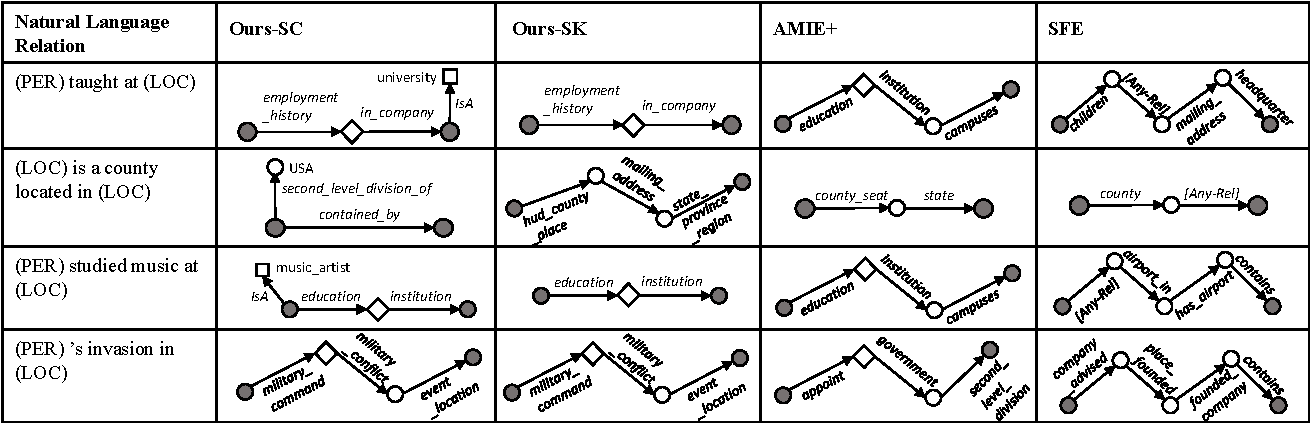
\includegraphics[width=1.0\columnwidth]{figure/schema/case-crop.eps}
    \centering
    \bicaption{不同的规则推导系统对四个复杂关系生成的代表性结构。}
    {Top structures produced by four systems on 4 complex relations.}
    \label{fig:schema-relation-example}
\end{figure*}

\figref{fig:schema-relation-example}列出了四个自然语言关系,
以及不同系统生成的最佳结构。
其中,圆点表示实体或变量,左右两个黑色圆点分别代表$x_{subj}$和$x_{obj}$。
方块代表知识库中的类型,菱形则代表用于维护多元关系的辅助节点。
%TODO: 如果篇幅不够,拿IJCAI的note来凑
从这些例子中可以发现,Ours-SC的模式图所具有的分支结构,可以带来更加精确的语义。
对比仅生成骨架的Ours-SK,带有限制的查询图在每个例子上都表达了几乎完全正确的语义。
另一方面,AMIE+和SFE输出的最佳结构不尽如人意。
AMIE+按照准确率对规则排序,因此总是倾向于更具体的规则,但牺牲了召回率。
同时随着规则长度提升至4甚至更高,AMIE+系统消耗了大量内存,无法返回任何结果。
SFE生成的规则中包含\textit{[Any-Rel]}代表任意谓词,因此可以生成更多灵活的路径作为特征,
但显然其中的大部分都不具有清晰的语义,人类难以直接理解。

作为补充实验,我们对Ours-SC和Ours-SK生成的模式图进行了人工测评。
对每一个自然语言关系,我们从中抽取出至多前5个概率值至少为0.05的模式图,
并由三位%熟悉Freebase结构的
标注者进行人工打分,
分值选择范围为\{0, 0.5, 1\},
分别代表 ``{不相关模式图}'' (骨架层次已出现语义偏离),
``{部分匹配}'' (骨架语义正确,但其余限制需要改善)以及
``{完全匹配}'' (骨架和限制的语义均无明显偏差)。
我们将三位标注者的打分进行平均,得到每一个模式图的标注分值,
并计算排名前$n$的所有模式图的平均分值,记做AvgSc@$n$。
三位标注者之间的Kappa系数为0.541,具有稳定的相关性。
\tabref{tab:average-score}列出了不同的AvgSc@$n$分值,
Ours-SC在骨架的基础上挖掘额外的语义限制,将结果提高了约13\%。

\begin{table}[ht]
	\centering
	\bicaption{模式图列表的AvgSc@$n$测评结果。}{AvgSc@$n$ results on top-ranked schemas.}
	\label{tab:average-score}
	\begin{tabular}{c|ccc}
		\hline
						&	n=1		&	n=3		&	n=5			\\
		\hline
		Ours-SK			&	0.44	&	0.37	&	0.34		\\
		Ours-SC			&	\textbf{0.47}	&	\textbf{0.40}	&	\textbf{0.38} \\
		\hline
	\end{tabular}
\end{table}


\subsubsection{主宾语预测任务测评}
主宾语预测任务的目标是预测三元组($e_{subj}$, $r$, $?$)或($?$, $r$, $e_{obj}$)
所缺失的宾语或主语。
测试集中的每一个三元组都对应两个这样的预测任务。
\eqnref{eqn:score-def}代表着给定一端实体,生成另一端未知实体的概率,
因此对每一个带有未知实体的待预测三元组,我们根据该公式计算生成不同实体的概率,
并衡量答案实体的概率排名高低。
我们在实验中使用了两个评价指标,分别为MRR和Hits@$n$,
前者衡量答案实体在所有预测任务中的平均排名,
后者关注在多少比例的预测任务中,答案实体的概率排在前$n$位。
不同的实验方法通过验证集的MRR分值进行独立调参。

以上对排名高低的衡量暗含着一个假设:除了答案实体之外,其余实体均为错误实体。
然而考虑到关系可能具有的一对多性质,对于一个待预测的三元组,
除了答案实体之外,还可能存在其它实体与给定的已知实体匹配,
严格来讲,这些实体虽然不同于唯一的答案,但也不应该算作错误。
因此,我们使用和TransE\cite{bordes2013translating}相同的设定,
在测评中引入两种不同的模式,分别为原始模式和过滤模式:
在过滤模式中,计算每个预测的答案实体排名时,均忽略不同于答案的其余正确实体,
因此过滤模式下,排名值可能会提高;而原始模式则不做任何的过滤。

%
%We perform the evaluation on FB15k under filtered setting \KZ{What is this
%setting? Never mentioned before?}.
%\figref{fig:trend-with-budget} shows how the MRR results
%\KQ{on validation set}, vary with the number of candidate schemas.
%From the results, we observe that:
%1) The MRR result increases with the number of candidate schemas in
%every setting, which indicates that larger number of candidates
%leads to a better model.
%2) Compare with strategies on candidate generation, use-whole-schema
%outperforms use-skeleton-only, demonstrating the capability of constraints
%to represent natural language relations.
%3) \KQ{random walk v.s. zero-one, need to get real results before the analysis.}
%
%%\KQ{Figure to be plotted: budget 1k~5k  *  4 different specifications.}
%\begin{figure}[th]
%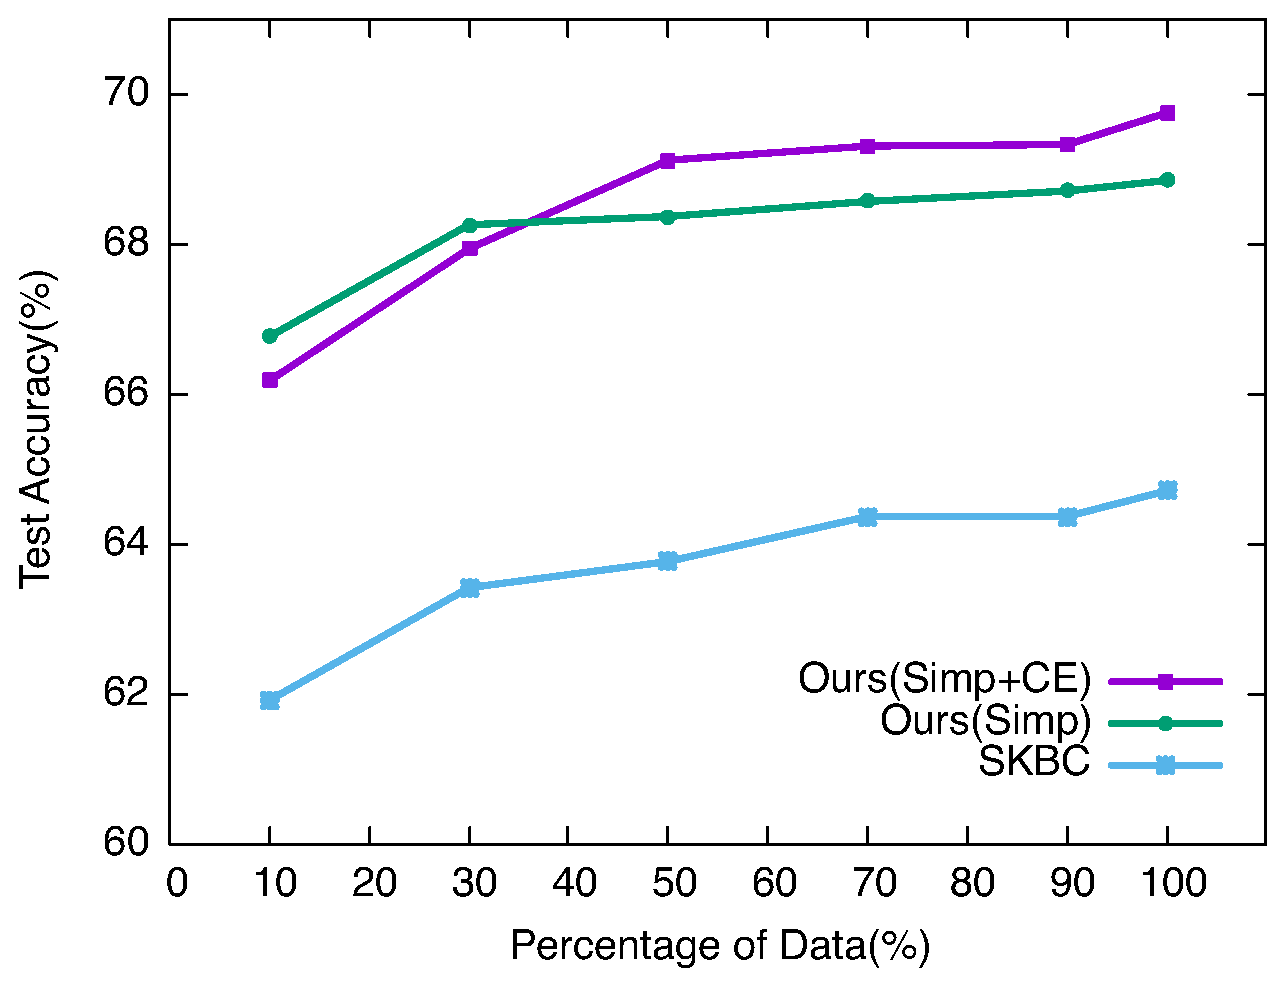
\epsfig{file=trend.eps, width=0.65\columnwidth}
%\centering
%\caption{
%	The trend of link prediction results on FB15k (filtered setting).
%	X axis: size of priority queue,
%	Y axis: MRR score. \KQ{content to be updated.}
%}
%\label{fig:trend-with-budget}
%\end{figure}

%We first evaluate our approach and state-of-the-art systems on PATTY-100 relations.
%Then we compare our approach with state-of-the-art models.
%\KQ{Need to say a little bit about the parameters we used here.}
%\tabref{tab:link-pred-patty} %and \tabref{tab:link-pred-filtered}
%shows the link prediction results on FB15k.

%\KZ{Due to memory issues of the code, SFE method failed to produce any result.
%This is a bit strange: you pick SFE as a comparison but it doesn't work for
%link prediction at all! Better fix this!}
%As we can see, our approach outperforms both embedding and
%other rule induction models.

我们使用FB15k作为知识库进行实验,并与其余模型进行比较。
在接下来的实验中,为了方便比较,
我们的模型同一参数$\gamma=10\%$,$\alpha=1e-4$,以及$\eta=0.1$,
对应着PATTY-100验证集上,在过滤模式下的最高MRR结果。
\tabref{tab:link-pred-patty}和\tabref{tab:link-pred-fb15k}
分别展示了在PATTY-100和FB15k-37数据集上的实验结果。
在两个数据集上,SFE模型的代码均碰到了内存问题,
因此表格中没有列出对应的结果。
对于PATTY-100中的关系,我们基于模式图的语义表示方法,
其效果优于其它用于比较的规则推导与知识库向量表示模型,
以及仅生成简单模式图的变种。
在FB15k-37数据集上,Ours-SC与Ours-SK的结果十分接近,
这主要是因为知识库上的一部分谓词具有等价形式,
例如$location.location.containedby$和$location.location.contains$
互为相反关系,对于这些关系,只需要依靠骨架结构就可以精确描述语义。
对比两张表格可以发现,对于所有不同的模型和实验模式,
自然语言关系上的主宾语预测结果都低于对应的知识库谓词上的结果。
%Comparing the results on different set of relations,
%the improvements on complex relations are much more significant than those
%on ordinary relations, indicating the usefulness of the extra constraints
%in representing complex relations.
%Besides, the link prediction results on natural language relations
%are relatively lower than
%those results evaluated on FB15k relations \cite{guo2016jointly}.
主要原因有两点:
1) FB15k-37上的每一个谓词平均包含接近千级别的训练三元组,
而PATTY-100中的每个关系平均只有115个训练数据;
2) 自然语言关系具有更多歧义,开放式信息抽取的结果会包含多种语义,
而且还要考虑抽取错误的情况,
相比之下,知识库上的谓词及三元组的制定经过了部分人工干预,因此歧义更少。


\begin{table}[b]
	\centering
	\bicaption{在PATTY-100上进行主宾语预测的测评结果。}{Link prediction results on PATTY-100 relations.}
	\label{tab:link-pred-patty}
	\begin{tabular}{c|ccc|ccc}
		\hline
				&	\multicolumn{3}{c|}{Raw}
				&	\multicolumn{3}{c}{Filtered}	\\
		\cline{2-7}	
				&	MRR	&	H@3	&	H@10
				&	MRR	&	H@3	&	H@10		\\
		\hline
		TransE
				&	0.112	&	12.4	&	27.1
				&	0.129	&	14.5	&	29.9	\\	%m1.75_lr0.10
		KALE
				&	0.112	&	12.5	&	25.4
				&	0.125	&	14.4	&	27.5	\\	%Test-base-k100-d0.15-ge0.02-gr10-filt.eval_KQ
		TEKE
				&	0.101	&	10.9	&	24.1
				&	0.114	&	12.6	&	26.3	\\
		HOLE
				&	0.109	&	10.5	&	23.3
				&	0.121	& 	12.3	&	25.8	\\	%log.hole_d100_m0.25_lr0.05
		%AMIE+
		%		&	0.119	&	23.5
		%		&	0.132	&	24.4	\\
		AMIE+
				&	0.148	&	16.5	&	29.3
				&	0.174	&	19.5	&	\textbf{31.9}	\\
		\hline
		Ours-SK
				&	0.169	&	18.2	&	29.3
				&	0.179	&	19.1	&	30.4	\\		%Blackhole
		Ours-SC
				&	\textbf{0.172}		&	\textbf{18.5}	&	\textbf{29.8}
				&	\textbf{0.185}		&	\textbf{19.9}	&	31.5	\\	%Blackhole
		\hline
	\end{tabular}
\end{table}

%\begin{table*}[ht]
%	\small
%	\centering
%	\caption{Link prediction results on FB15k (raw setting).}
%	\begin{tabular}{|c|ccccc|ccccc|ccccc|}
%		%\toprule
%		\hline
%				&	\multicolumn{5}{c|}{Complex relations}
%				&	\multicolumn{5}{c|}{Ordinary relations}
%				&	\multicolumn{5}{c|}{Overall}	\\
%		\cline{2-16}	
%		\multirow{2}{*}{}	&	\multirow{2}{*}{MRR}	&	\multirow{2}{*}{MED}	&	\multicolumn{3}{c|}{Hit@n(\%)}
%							&	\multirow{2}{*}{MRR}	&	\multirow{2}{*}{MED}	&	\multicolumn{3}{c|}{Hit@n(\%)}
%							&	\multirow{2}{*}{MRR}	&	\multirow{2}{*}{MED}	&	\multicolumn{3}{c|}{Hit@n(\%)}	\\
%				&	&	&	3	&	5	&	10	
%				&	&	&	3	&	5	&	10	
%				&	&	&	3	&	5	&	10	\\
%		\hline
%		TransE
%				&	0.089	&	75.0	&	11.7	&	17.2	&	23.2
%				&	0.081	&	66.0	&	 8.1	&	12.1	&	19.6
%				&	0.082	&	68.0	&	 8.9	&	13.2	&	20.4	\\
%		KALE	
%				&	0.142	&	47.0	&	17.5	&	23.4	&	30.5
%				&	0.104	&	42.0	&	11.2	&	16.0	&	24.0
%				&	0.112	&	\textbf{43.0}	&	12.5	&	17.6	&	25.4	\\
%		TEKE	
%				&	0.119	&	68.4	&	14.7	&	19.5	&	27.6
%				&	0.096	&	57.2	&	9.8  	&	14.6	&	23.1
%				&	0.101	&	59.0	&	10.9	&	15.7	&	24.1	\\
%		HOLE
%				&	0.153	&	55.0	&	16.0	&	20.5	&	27.4
%				&	0.097	&	51.0	&	 9.1	&	13.9	&	22.2
%				&	0.109	&	52.0	&	10.5	&	15.4	&	23.3	\\
%		%\hline
%		%SFE-AnyRel
%		%SFE-OneSide
%		AMIE+
%				&	0.164	&	76.3	&	18.2	&	21.9	&	26.6
%				&	0.107	&	68.3	&	11.3	&	15.8	&	22.6
%				&	0.119	&	69.5	&	12.7	&	17.1	&	23.5	\\
%		Ours
%				&	0.225	&	42.5	&	24.3	&	27.8	&	34.7
%				&	0.158	&	43.0	&	16.9	&	21.0	&	28.5
%				&	\textbf{0.172}	&	\textbf{43.0}	&	\textbf{18.5}	&	\textbf{22.5}	&	\textbf{29.8}	\\
%		\hline
%	\end{tabular}
%	\label{tab:link-pred-raw}
%\end{table*}

\begin{table}[tbh]
	\centering
	\bicaption{在FB15k-37上进行主宾语预测任务的测评结果。}{Link prediction results on FB15k-37 relations.}
	\label{tab:link-pred-fb15k}
	\begin{tabular}{c|ccc|ccc}
		\hline
				&	\multicolumn{3}{c|}{Raw}
				&	\multicolumn{3}{c}{Filtered}	\\
		\cline{2-7}	
				&	MRR	&	H@3	&	H@10
				&	MRR	&	H@3	&	H@10	\\
		\hline
		TransE
				&	0.310			&	39.3	&	53.2
				&	0.394	&	52.5	&	65.0	\\	%log.transe_m2.00_lr0.10.train_lp
		KALE
				&	0.342	&	40.6	&	53.0
				&	0.410	&	48.7	&	60.6	\\	%Test-KALE-1110-k100-d0.12-rd0.12-ge0.05-gr10-w1(0.1)-w2(1)-w3(0)-w4(0)-filt.eval_KQ
		TEKE
				&	0.288	&	35.7	&	49.2
				&	0.339	&	43.0	&	56.5	\\
		HOLE
				&	0.234	&	26.7	&	39.5
				&	0.323	& 	36.5	&	50.5	\\	%log.hole_m0.25_lr0.10.train_lp
		AMIE+
				&	0.395	&	46.1	&	53.7
				&	0.562	&	60.0	&	68.9	\\
		\hline
		Ours-SK
				&	0.425	&	47.8	&	55.6
				&	0.664	&	68.8	&	73.0	\\		%Darkstar
		Ours-SC
				&	\textbf{0.427}		&	\textbf{48.1}	&	\textbf{55.7}
				&	\textbf{0.671}		&	\textbf{69.3}	&	\textbf{73.3}	\\		%Darkstar
		\hline
	\end{tabular}
\end{table}

%\begin{table*}[ht]
%	\small
%	\centering
%	\caption{Link prediction results on FB15k (filtered setting).}
%	\begin{tabular}{|c|ccccc|ccccc|ccccc|}
%		%\toprule
%		\hline
%				&	\multicolumn{5}{c|}{Complex relations}
%				&	\multicolumn{5}{c|}{Ordinary relations}
%				&	\multicolumn{5}{c|}{Overall}	\\
%		\cline{2-16}	
%		\multirow{2}{*}{}	&	\multirow{2}{*}{MRR}	&	\multirow{2}{*}{MED}	&	\multicolumn{3}{c|}{Hit@n(\%)}
%							&	\multirow{2}{*}{MRR}	&	\multirow{2}{*}{MED}	&	\multicolumn{3}{c|}{Hit@n(\%)}
%							&	\multirow{2}{*}{MRR}	&	\multirow{2}{*}{MED}	&	\multicolumn{3}{c|}{Hit@n(\%)}	\\
%				&	&	&	3	&	5	&	10	
%				&	&	&	3	&	5	&	10	
%				&	&	&	3	&	5	&	10	\\
%		\hline
%		TransE
%				&	0.097	&	69.0	&	13.0	&	18.7	&	25.0
%				&	0.092	&	62.0	&	 9.7	&	14.2	&	22.2
%				&	0.094	&	63.0	&	10.4	&	15.2	&	22.8	\\
%		KALE	
%				&	0.153	&	43.0	&	19.9	&	25.5	&	32.5
%				&	0.118	&	39.0	&	12.9	&	18.0	&	26.1
%				&	0.125	&	\textbf{39.0}	&	14.4	&	19.6	&	27.5	\\
%		TEKE	
%				&	0.129	&	64.3	&	16.2	&	21.4	&	29.1
%				&	0.109	&	52.7	&	11.7	&	16.9	&	25.6
%				&	0.114	&	54.0	&	12.6	&	17.9	&	26.3	\\
%		HOLE
%				&	0.162	&	50.5	&	17.4	&	21.8	&	29.0
%				&	0.109	&	47.0	&	10.9	&	16.1	&	24.9
%				&	0.121	&	47.0	&	12.3	&	17.3	&	25.8	\\
%		%\hline
%		%SFE-AnyRel
%		%SFE-OneSide
%		AMIE+
%				&	0.180	&	73.8	&	18.6	&	22.4	&	27.5
%				&	0.120	&	63.5	&	12.5	&	17.0	&	23.6
%				&	0.132	&	65.0	&	13.8	&	18.2	&	24.4	\\
%		Ours
%				&	0.237	&	41.0	&	25.2	&	29.1	&	35.5
%				&	0.171	&	40.0	&	18.4	&	22.4	&	30.5
%				&	\textbf{0.185}	&	40.0	&	\textbf{19.9}	&	\textbf{23.8}	&	\textbf{31.5}	\\
%		\hline
%	\end{tabular}
%	\label{tab:link-pred-filtered}
%\end{table*}





\subsubsection{三元组分类任务测评}
三元组分类任务的目标是预测一个未知三元组($e_1$, $r$, $e_2$)是否描述了一个正确的客观事实。
考虑到这是个二分类任务,测试数据中需要包含负样本三元组,
因此我们使用和KALE\cite{guo2016jointly}相同的生成策略,
对测试集和验证集中的每个三元组生成10个不同的负样本,
其中5个三元组替换了主语,另外5个替换了宾语。
为了保证负样本不至于显得过于错误,
我们保证用于替换的主语(或宾语)都曾出现在目标关系的某个已知三元组的同样位置上。

对于每一个目标关系,我们通过\eqnref{eqn:likelihood-def}计算各个未知三元组的似然值,
以此作为置信度对所有测试集的所有正负样本进行排序。
我们使用FB15k作为知识库进行了实验,
并使用MAP(Mean Average Precision)作为测评指标,
衡量不同的模型在三元组分类任务上的效果。
%TODO: 找个地方说一下评价指标
\tabref{tab:triple-clsf}列出了PATTY-100和FB15k-37数据集上的效果,
我们的模型在两个数据集上均大幅度优于其它方法。
此外我们发现,仅生成简单模式图的方法效果要优于生成完整模式图的做法。
我们对实验数据进行了分析,
造成这个现象的原因源于负样本生成方式的天然缺陷。
例如对于 ``father of'' 关系,我们期望负样本中能包含表示母子关系的实例,
识别这种负样本需要较高难度,必须依靠额外限制才能和正样本进行区分。
然而,负样本的生成方式决定了主语只能替换为某个随机小孩的父亲,
判断三元组正确与否主要依靠骨架的正确性,
因而很难体现模式图的额外限制为给语义理解带来的优势,
减少候选模式图的数量和复杂度反而能得到更好的效果。


%(what we generated in the current experimental setting)
%as negative data makes the classification problem harder, and shows the value of constraints.
%While in link prediction, the constraints play an important role to 
%rank positive entities higher.
%Moreover, we find that there's almost no difference
%between our two variances on FB15k-37, that's not unexpected because skeletons
%are enough to represent the majority of these predicates.


%Observing results of each model, it's interesting to find that all rule induction models
%performs much better than embedding techniques, which reveals us that
%explicit semantic feature mining could help to find more precise representations,
%especially when the training data is small.
%Ours-SC outperforms the other embedding methods on PATTY-100 dataset, demonstrating the
%importance of constraints. However, the gap could be bigger if the negative triples
%are generated to distinguish the constraints, e.g., for father-of relation,
%using a child's own mother instead of a random father or a random mother as negative data.

\begin{table}[tbh]
	\centering
	\bicaption{三元组分类任务的MAP测评结果。}{MAP results on triple classification task.}
	\begin{tabular}{c|cc}
		%\toprule
		\hline
							& PATTY-100	&	FB15k-37 	\\
        \hline
		TransE				&	0.304	&	0.666	\\	% m0.25, lr0.05	|	m1.00, lr0.10
		KALE				&	0.309	&	0.654	\\
		TEKE				&	0.282	&	0.631	\\
		HOLE				&	0.308	&	0.680	\\	% m0.25, lr0.20	|	m0.20, lr0.10
		SFE					&	0.329	&	0.621	\\	% due to data shrinking ...
		AMIE+				&	0.226	&	0.730	\\	
		\hline
		Ours-SK				&	\textbf{0.408}	&	\textbf{0.804}	\\	
		Ours-SC				&	0.403	&	0.803	\\
		\hline
	\end{tabular}
	\label{tab:triple-clsf}
\end{table}



\subsubsection{错误分析}

%\figref{fig:relation-example} shows the paraphrasing results of
%selected relations.
%Show a case-by-case P/R/F1/RR?
%The results of top-ranked schemas show us that our paraphrasing system
%is able to produce concrete and precise structural representations.
对于一些自然语言关系,我们的模型可能难以寻找出较为正确的模式图。
我们对结果进行了分析,并总结出以下几类主要错误。

1. 开放式信息抽取提供的关系三元组存在错误。
考虑到PATTY主要利用依存语法分析对句子进行关系识别,
语法分析本身的偏差将导致生成错误的三元组。
例如对于关系\textit{``served as''},给定句子
\textit{``Dennison served as the 24th Governor of Ohio and as U.S. Postmaster General ...''},
PATTY提取的实体对(William Dennison Jr., Ohio)
有误,正确的宾语应为``Governor of Ohio'' 。

2. PATTY数据集中,每个关系实际代表着一个关系同义集,即由多个具有相似结构的关系组成的组合,
这导致部分关系同义集混入了语法相似但语义不同的关系,产生本不存在的歧义。
以PATTY中的关系同义集\textit{``'s wife''}为例,
其中混入了少部分可能由\textit{``the wife of''}产生的三元组,其中主语为妻子,宾语反而为丈夫。
%由于PATTY并未提供原句,因此不能直接对关系同义集里的内容进行过滤。
在混入的三元组干扰下,模型会误以为该关系的准确语义为不带有性别限制的配偶关系,
因此正确的模式图很难获得较高的概率。
%These instances are due to another pattern in the synset,
%\textit{``the wife of''}, which gives the exact opposite semantics.
%though our system is able to filter out noisy instances, the learned schema
%distribution would be affected if the percentage of noisy data is large.

3. 对于部分关系,知识库本身缺乏用于描述其语义的谓词。
对于一些琐碎的自然语言关系例如\textit{``talk to''},知识库显然不包含这类事实。
但即便对于一些不那么琐碎的关系,知识库依然可能缺乏必要的谓词。
例如关系\textit{``(singer) performed in (LOC)''}	% synset 0246
描述的是歌手和演唱会举办地的联系,但Freebase中并不包含类似于
\textit{place\_visited}或\textit{hold\_concerts\_in}的谓词,
因此难以通过已有知识表示目标关系的语义。

4. 由于搜索空间的限制,部分有意义的模式图无法在候选生成步骤被过滤。
例如关系\textit{``(actor) starring with (actor)''},
由于Freebase通过辅助节点(Mediator)维护多元关系,
这使得最合适的骨架\footnote{
骨架具有$actor \rightarrow med. \rightarrow film \rightarrow med. \rightarrow actor$
形式,其中$med.$为辅助节点。}长度为4,并不满足候选生成的骨架长度限制,因此模型无法得到这样的模式图。

%\KZ{This is why I said we should evaluate the impact of $\tau$.}
%
%\KZ{After reading this paper, one thing that puzzles me is that why is this
%method called paraphrasing natural language relations to knowledge base? The
%approach you are proposing can be used for ordinary KB completion task, right?
%In other words we are not making use of the natural language feature at all.
%I think perhaps we can include some experiments you did with NL features to
%show that NL features are not necessary and explain why. This will clear the
%doubt of some readers.}




\section{小结}
This work mines the equivalence between natural language relations and structured 
knowledge known as schemas.  It generalizes the simple path representation 
by adding constraints along the path and thus support more complex semantics.
Experiments show that schema representation is able to describe the concrete 
and precise semantic meaning. Schemas thus learned have higher quality than
those learned by existing rule induction approaches. Our approach can also be applied
to the traditional knowledge base completion problem and yield good results. 
%and performs as well as the state-of-the-art methods on ordinary relations.
%To the best of our knowledge, this is the first attempt to directly model complex NL relations in knowledge bases.
%We have observed that this data-driven approach benefits from 
%increasing amount of training data, but it's sensitive to the noisy pairs in the input.
%Future research may aim at designing a self-adaptive algorithm to detect and filter noisy data
%from relation instances, and leverage the structural knowledge to improve performance of QA systems.
%
%Future direction of this research includes schema inference from
%small data sets, efficient generation of
%more complex schemas, including comparative and aggregative constraints, 
%and the exploration of other features during
%schema weighting.
%

本章的研究成果已发表于2017年国际会议International Joint Conference on Artificial Intelligence
(IJCAI2017),论文题目为
``A Data-Driven Approach to Infer Knowledge Base Representation for Natural Language Relations''。
